% vim:autoindent:set textwidth=78:

\section{Trabajar con datos vectoriales}\label{label_workingvector}
\index{vector layers|(}

% when the revision of a section has been finalized,
% comment out the following line:
%\updatedisclaimer


QGIS admite datos vectoriales en distintos formatos, incluyendo aquellos soportados por el proveedor de datos de la biblioteca OGR, tales como archivos shape de ESRI,
\index{shapefiles}\index{ESRI!shapefiles}\index{SHP files}
MapInfo MIF (formato de intercambio)\index{MIF files}\index{MapInfo!MIF files}
y MapInfo TAB (formato nativo).\index{TAB files}\index{MapInfo!TAB files}
Puede encontrar una lista de los formatos vectoriales admitidos por OGR en el Ap\'endice~\ref{appdx_ogr}.

QGIS también admite capas de PostGIS\index{PostGIS}\index{PostgreSQL!PostGIS} en una base de datos PostgreSQL usando el proveedor de datos PostgreSQL. El soporte para tipos de datos adicionales (ej. texto delimitado) se provee a trav\'es de proveedores de datos adicionales.\index{delimited text}

Esta secci\'on describe cómo trabajar con diferentes formatos comunes:
archivos shape de ESRI, capas de PostGIS y capas de SpatialLite. Muchas de las funciones disponibles en QGIS trabajan de la misma forma, independientemente de la fuente de datos vectoriales.
Esto es así por dise\~no e incluye las funciones de identificar, seleccionar, etiquetar y de atributos.

La forma de trabajar con vectores de GRASS se describe en la Secci\'on \ref{sec:grass}.

\subsection{Archivos shape de ESRI}
\index{vector layers!ESRI shapefiles}
\index{shapefiles}
\index{ESRI!shapefiles}
\index{SHP files}

El formato de archivo vectorial estándar usado en QGIS es el archivo shape de ESRI. El soporte se provee a trav\'es de la biblioteca OGR Simple Feature (\url{http://www.gdal.org/ogr/})
\index{OGR}. Un archivo shape en realidad consiste en m\'ultiples archivos. Se requieren al menos los tres siguientes:
\index{shapefile!format}

\begin{itemize}
\item \filename{.shp} archivo que contiene las geometr\'{\i}as del objeto espacial.
\item \filename{.dbf} archivo que contiene los atributos en formato dBase.
\item \filename{.shx} archivo de \'{\i}ndices.
\end{itemize}

Los archivos shape también pueden incluir un archivo con un sufijo \filename{.prj}, que contiene la informaci\'on de la proyecci\'on. Aunque es muy \'util tener un archivo de proyecci\'on, no es obligatorio. Un conjunto de datos shape puede contener archivos adicionales. Para mayores detalles vea la especificaci\'on t\'ecnica de ESRI en  \url{http://www.esri.com/library/whitepapers/pdfs/shapefile.pdf}
\index{shapefile!specification}.

\subsubsection{Cargar un archivo shape}\label{sec:load_shapefile}

\begin{figure}[ht]
   \begin{center}
   \caption{Di\'alogo Abrir capa vectorial \nixcaption}\label{fig:addvectorlayer}\smallskip
   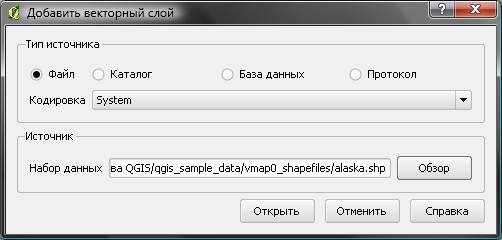
\includegraphics[clip=true, width=12cm]{addvectorlayerdialog}
\end{center} 
\end{figure}

\begin{figure}[ht]
   \begin{center}
   \caption{Di\'alogo Abrir una capa vectorial de OGR \nixcaption}\label{fig:openshapefile}\smallskip
   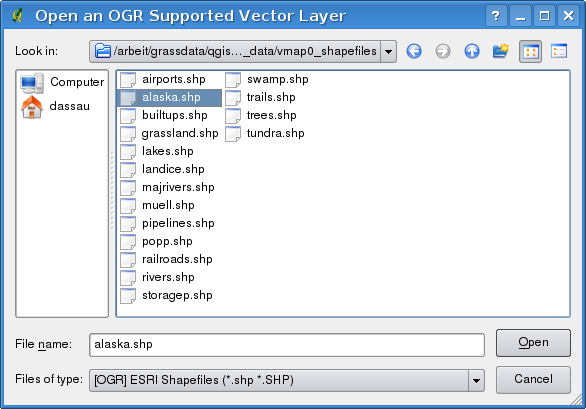
\includegraphics[clip=true, width=14cm]{shapefileopendialog}
\end{center} 
\end{figure}

\begin{figure}[ht]
   \begin{center}
   \caption{QGIS con un archivo shape de Alaska cargado \nixcaption}\label{fig:loadedshapefile}\smallskip
   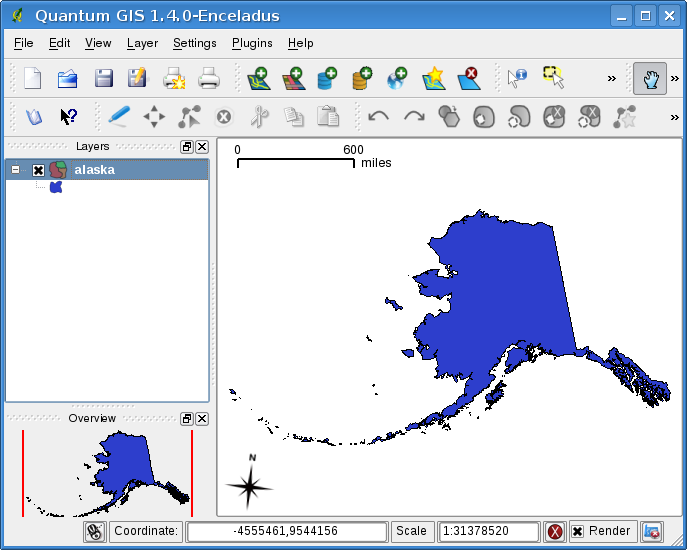
\includegraphics[clip=true, width=16cm]{shapefileloaded}
\end{center} 
\end{figure}

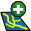
\includegraphics[width=0.7cm]{mActionAddNonDbLayer} Para cargar un archivo shape, inicie
QGIS y haga clic en el bot\'on \toolbtntwo{mActionAddNonDbLayer}{A\~nadir capa vectorial} de la barra de herramientas
\index{shapefile!loading} o simplemente presione la tecla \keystroke{V}. Esto abrir\'a una nueva ventana (vea la Figura \ref{fig:addvectorlayer}).

De los botones de selecci\'on disponibles marque \radiobuttonon{Archivo}. Pulse \button{Explorar}. Eso abrir\'a un di\'alogo de abrir archivo estándar (vea la Figura \ref{fig:openshapefile}) que permite navegar el sistema de archivos y cargar un archivo shape o cualquier otra fuente de datos admitida. 
La caja de selecci\'on \selectstring{Ficheros de tipo}{\ldots} permite preseleccionar algunos formatos de archivos OGR soportados.

Puede seleccionar también el tipo de codificaci\'on deseado para el archivo shape.

Seleccionando un archivo shape de la lista y haciendo clic en \button{Abrir} lo carga dentro de QGIS. La Figura
\ref{fig:loadedshapefile} muestra QGIS después de cargar el archivo \filename{alaska.shp}.


\begin{Tip}\caption{\textsc{Colores de la capa}}
\qgistip{Cuando agrega una capa al mapa, se le asigna un color de manera aleatoria. Cuando se
agrega más de una capa al mismo tiempo, se le asignan diferentes colores a cada capa. }
\end{Tip}

Una vez cargado, puede hacer acercamientos o alejamientos al archivo shape usando las herramientas de navegaci\'on del mapa.
Para cambiar la simbolog\'ia de la capa, abra el di\'alogo \dialog{Propiedades de la capa} haciendo doble clic en el nombre de la capa o haciendo clic derecho en el nombre de la capa en la leyenda y eligiendo \dropmenuopt{Propiedades} del men\'u emergente. Vea la  Secci\'on \ref{sec:symbology} para más informaci\'on sobre cómo configurar la simbolog\'{\i}a de las capas vectoriales.
  
\subsubsection{Mejorar el rendimiento}

Para mejorar el rendimiento del dibujado de un archivo shape, puede crear un \'{\i}ndice espacial. Un \'{\i}ndice espacial \index{spatial index!shapefiles} mejorar\'a la velocidad en las operaciones de acercar, alejar y desplazar. Los \'{\i}ndices espaciales usados por QGIS tienen una extensi\'on \filename{.qix}.

Use estos pasos para crear el \'{\i}ndice:

\begin{itemize}
\item Cargue un archivo shape.
\item Abra el di\'alogo \dialog{Propiedades de la capa} haciendo doble clic en el nombre del archivo shape en la leyenda o haciendo clic derecho en el nombre de la capa en la leyenda y eligiendo \dropmenuopt{Propiedades} del men\'u emergente.
\item En la pesta\~na \tab{General} haga clic en el bot\'on \button{Crear \'indice espacial}.
\end{itemize}

\subsubsection{Cargar una capa de MapInfo}
\index{vector layers!MapInfo}

Para cargar una capa de MapInfo, haga clic en el bot\'on  \toolbtntwo{mActionAddNonDbLayer}{A\~nadir capa vectorial}
de la barra de herramientas o presione la tecla \keystroke{V}, cambie el filtro de tipo de archivo a
\selectstring{Ficheros de tipo}{[OGR] MapInfo (*.mif
*.tab *.MIF *.TAB)} y seleccione la capa que desea cargar.

\subsubsection{Cargar un ArcInfo Binary Coverage}
\index{vector layers!ArcInfo Binary Coverage}

Para cargar un ArcInfo binary coverage haga clic en el bot\'on  
\toolbtntwo{mActionAddNonDbLayer}{A\~nadir capa vectorial} de la barra de herramientas
o presione la tecla \keystroke{V} para abrir el di\'alogo 
\dialog{A\~nadir capa vectorial}.  Seleccione \radiobuttonon{Directorio}. Cambie a \selectstring {Tipo}{Arc/Ingo Binary Coverage}. 
Navegue al directorio que contiene los archivos de coberturas y selecci\'onelo.

De forma similar, puede cargar vectores basados en directorio como el formato UK National Transfer, as\'{\i} como el 
formato raw TIGER del US Census Bureau.

\subsection{Capas PostGIS}
\index{vector layers!PostGIS|see{PostGIS}}
\index{PostGIS!layers}
\label{label_postgis} 

Las capas de PostGIS se almacenan en una base de datos PostgreSQL. Las ventajas de PostGIS
son indexamiento espacial, filtrado y las capacidades de consulta que provee. Usando PostGIS, funciones
vectoriales tales como seleccionar e identificar funcionan mucho más eficazmente que con
capas OGR en QGIS.

Para usar capas de PostGIS debe:\index{PostgreSQL!loading layers}
\begin{itemize}
\item Crear una conexi\'on almacenada en QGIS a la base de datos PostgreSQL (si no ha sido
previamente definida).\index{PostgreSQL!connection}
\item Conectarse a la base de datos.
\item Seleccionar la capa a agregar al mapa.
\item Opcionalmente proveer una clausula SQL \usertext{where}
para definir qué caracter\'{\i}sticas cargar desde la capa.
\item Cargar la capa.
\end{itemize}

\subsubsection{Crear una conexi\'on almacenada}\index{PostgreSQL!connection}\label{sec:postgis_stored}

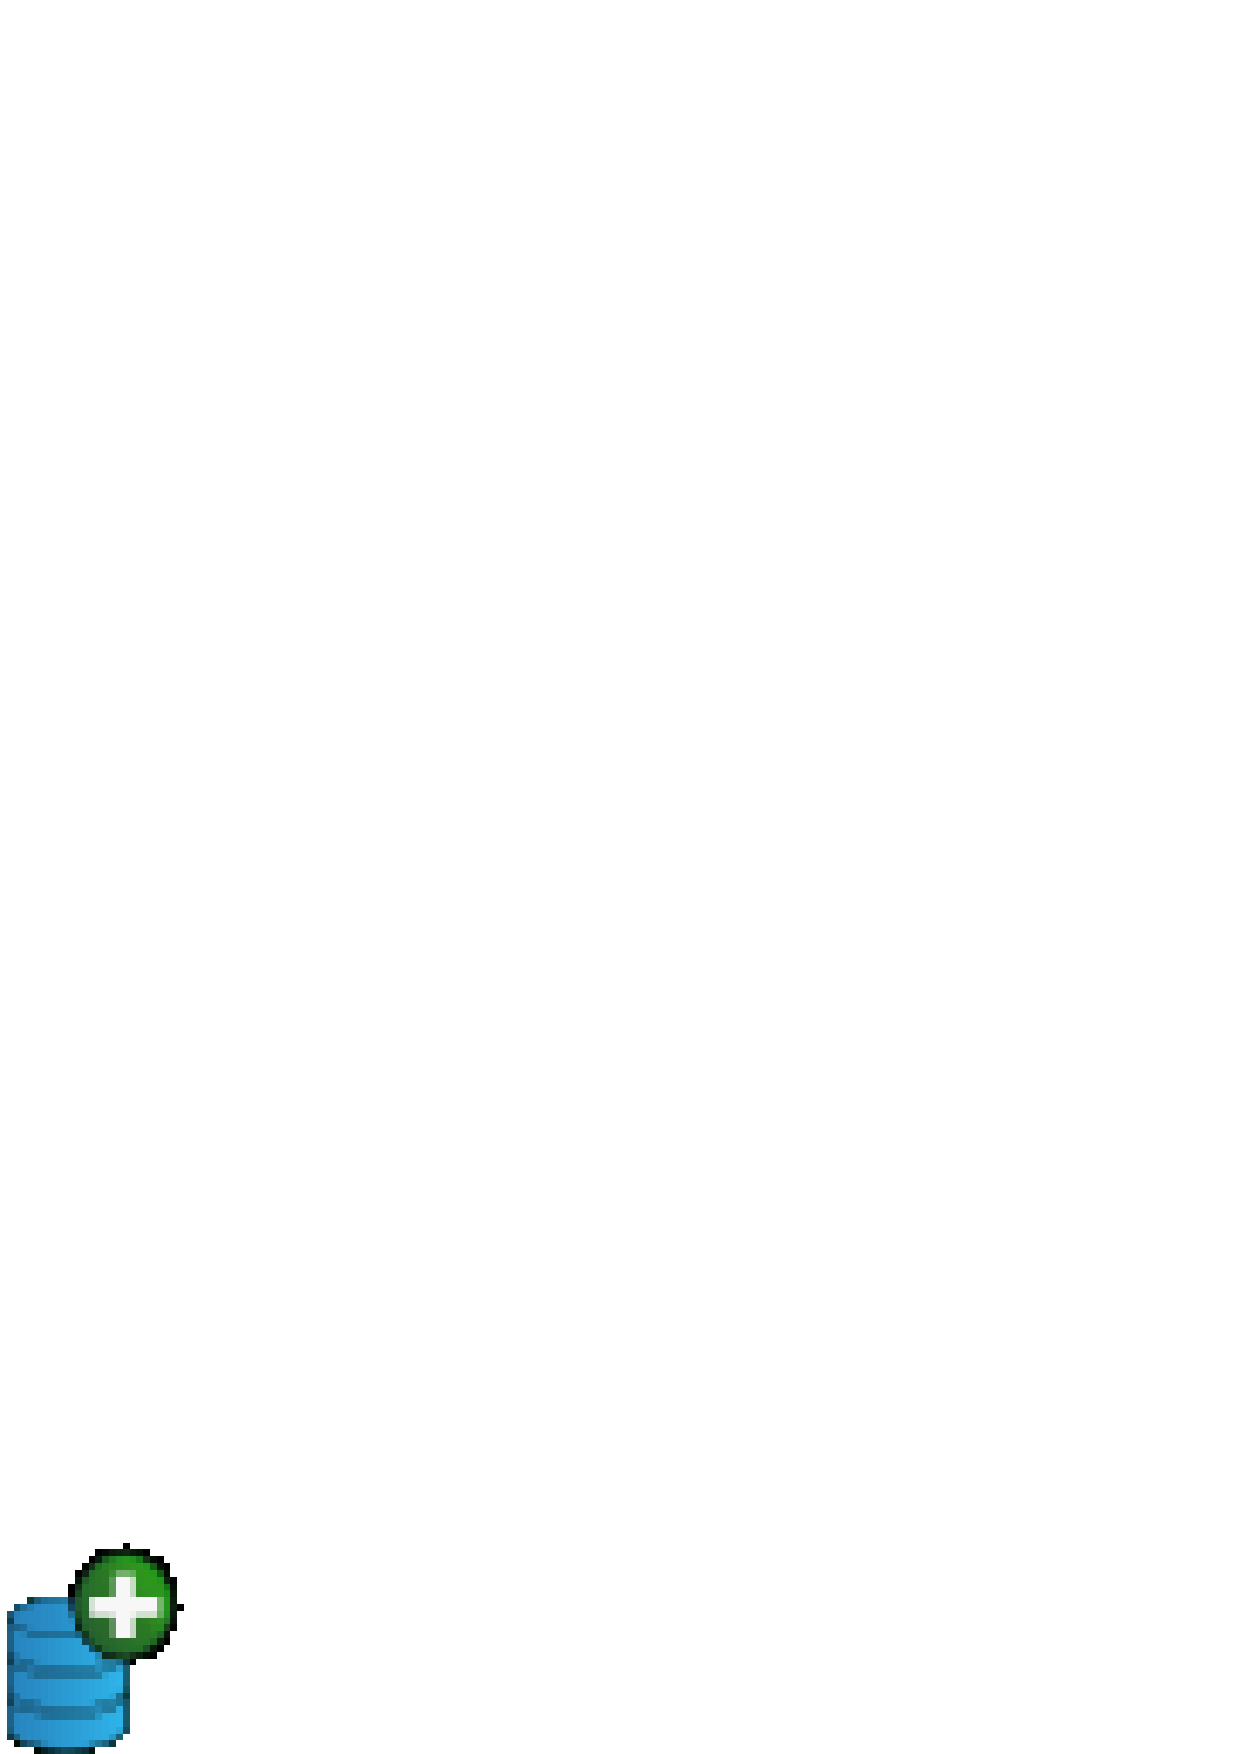
\includegraphics[width=0.7cm]{mActionAddLayer} La primera vez que utilize un conjunto de datos PostGIS, debe crear una conexi\'on a la base de datos PostgreSQL que contiene los datos. Comienze haciendo clic en el bot\'on \toolbtntwo{mActionAddLayer}{A\~nadir capa de PostGIS} de la barra de herramientas, seleccionando la opci\'on 
\dropmenuopttwo{mActionAddLayer}{A\~nadir capa de PostGIS...} del men\'u \mainmenuopt{Capa} o presionando la tecla \keystroke{D}. También puede abrir el di\'alogo \dialog{A\~nadir capa vectorial} y seleccionar \radiobuttonon{Base de datos}.
Se abrir\'a el di\'alogo \dialog{A\~nadir tabla(s) PostGIS}. Para acceder al administrador de conexiones \index{PostgreSQL!connectionmanager}, haga clic en el bot\'on \button{Nueva} para mostrar el di\'alogo  \dialog{Crear una nueva conexi\'on a PostGIS}. Los par\'ametros requeridos para una conexi\'on se muestran en la tabla \ref{tab:postgis_connection_parms}.

\begin{table}[ht]\index{PostgreSQL!connection parameters}
\centering
\caption{Par\'ametros de conexi\'on a PostGIS}\label{tab:postgis_connection_parms}\medskip
 \begin{tabular}{|l|p{5in}|}
\hline Nombre & Un nombre para esta conexi\'on. Puede ser el mismo que \textsl{Base de datos}.
\\
\hline Servidor \index{PostgreSQL!host}
& Nombre del servidor de bases de datos. Este debe ser un nombre de servidor que pueda ser resuelto igual al que usaría
para abrir una conexi\'on telnet o hacer un ping al servidor. Si la base de datos est\'a 
en la misma computadora que QGIS, simplemente introduzca 'localhost' aqu\'{\i}. \\
\hline Base de datos \index{PostgreSQL!database} & Nombre de la base de datos.  \\
\hline Puerto \index{PostgreSQL!port}& N\'umero del puerto en el que el servidor 
de base de datos PostgreSQL escucha. El puerto predeterminado es el 5432.\\
\hline Nombre de usuario \index{PostgreSQL!username}& El nombre de usuario se usa para iniciar sesi\'on
en la base de datos. \\
\hline Contrase\~na \index{PostgreSQL!password}& Contrase\~na usada por
\textsl{Nombre de usuario} para conectarse a la base de datos.\\
\hline Modo SSL \index{PostgreSQL!sslmode}& Como ser\'a negociada la conexi\'on SSL con el servidor. Estas son las opciones: 
\begin {itemize}
\item desactivar: sólo intentar una conexi\'on SSL no encriptada;
\item permitir: intentar una conexi\'on sin SSL, si ésto falla, intentar una conexi\'on SSL;
\item preferir (predeterminada): intentar una conexi\'on SSL, si falla, intentar una conexi\'on no-SSL;
\item requerir: solo intentar una conexi\'on SSL.
\end {itemize}
Tenga en cuenta que se pueden alcanzar aumentos masivos en la velocidad de dibujado de capas PostGIS desactivando SSL en el editor de conexiones. \\
\hline
\end{tabular}
\end{table}

Opcionalmente puede activar las siguientes casillas:

\begin{itemize}
\item \checkbox{Guardar contrase\~na}
\item \checkbox{Sólo buscar en la tabla geometry\_columns}
\item \checkbox{Sólo buscar en el esquema 'public'}
\end{itemize}

Una vez que ha establecido todos los par\'ametros y opciones, puede probar la conexi\'on haciendo clic 
en el bot\'on \button{Probar conexi\'on} \index{PostgreSQL!connection!testing}.

\begin{Tip}\caption{\textsc{Configuraciones de Usuario y Seguridad de QGIS}}\index{settings}\index{security}
\qgistip{Sus configuración personalizada para QGIS se almacena dependiendo del sistema
operativo. En \nix, la configuración se almacena en su directorio home en
\filename{.qt/qgisrc}. En \win, la configuración se almacena en el registro. Dependiendo de su
ambiente de computo, almacenar contrase\~nas en su configuración de QGIS puede ser
un riesgo de seguridad.
}
\end{Tip}

\subsubsection{Cargar una capa PostGIS}\index{PostgreSQL!loading layers}

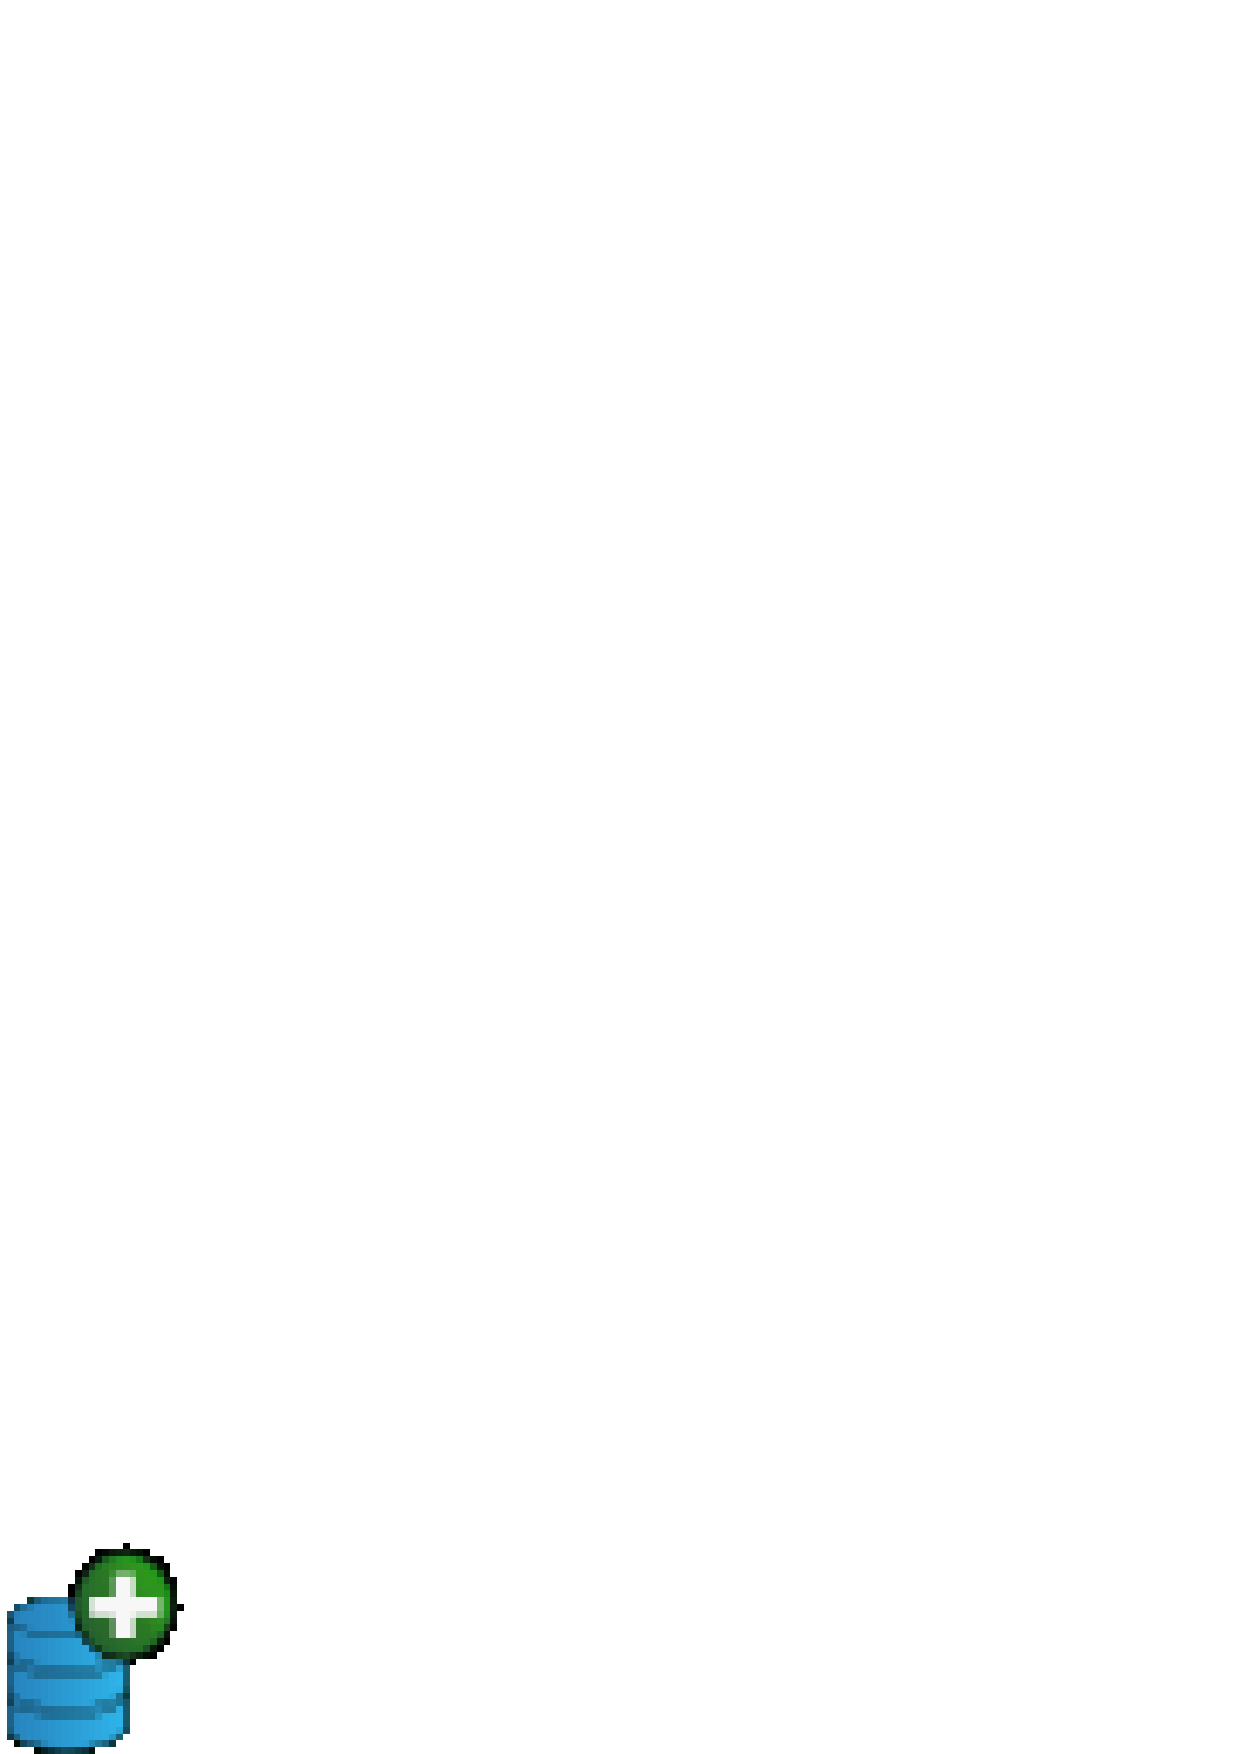
\includegraphics[width=0.7cm]{mActionAddLayer} Una vez que tiene una o más
conexiones definidas, puede cargar capas desde la base de datos PostgreSQL. Claro
que esto requiere tener datos en PostgreSQL. Vea la secci\'on
\ref{sec:loading_postgis_data} para una discusi\'on sobre importar datos dentro de la
base de datos. 

Para cargar una capa de PostGIS, realice los siguientes pasos:

\begin{itemize}
\item Si el di\'alogo \dialog{A\~nadir tabla(s) PostGIS} no esta abierto aún, haga clic en el bot\'on
\toolbtntwo{mActionAddLayer}{A\~nadir capa PostGIS} de la barra de herramientas.
\item Elija la conexi\'on de la lista desplegable y haga clic en \button{Conectar}.
\item Encuentre la capa que desea agregar en la lista de capas disponibles.
\item Seleccionela haciendo clic en ella. Puede seleccionar m\'ultiples capas presionando
la tecla \keystroke{shift} mientras hace clic. Vea la secci\'on \ref{sec:query_builder} para
informaci\'on sobre usar el Constructor de cronsultas de PostgreSQL para definir con más precisi\'on la capa.
\item Clic en el bot\'on \button{A\~nadir} para agregar una capa al mapa.
\end{itemize}

\begin{Tip}\caption{\textsc{Capas PostGIS}}
\qgistip{Normalmente una capa PostGIS es definida por una entrada en la tabla
geometry\_columns. Desde la versi\'on \OLD % should be 0.9.0 
hacia arriba, QGIS puede cargar capas que no tienen una entrada
en la tabla geometry\_columns. Esto incluye tablas y vistas.
La definici\'on de una vista espacial provee poderosos medios para visualizar sus datos. Rem\'{\i}tase
a su manual de PostgreSQL para informaci\'on sobre creaci\'on de vistas.}
\end{Tip}

\subsubsection{Algunos detalles acerca de capas PostgreSQL}\label{sec:postgis_details}
\index{PostgreSQL!layer details}

Esta secci\'on contiene algunos detalles de como QGIS accesa capas PostgreSQL. La mayor\'{\i}a de las veces QGIS deber\'{\i}a simplemente proveerle una lista de tablas de la base de datos que pueden ser cargadas, y cargarlas cuando sea necesario. Sin embargo, si tiene problemas cargando una tabla PostgreSQL en QGIS, la siguiente informaci\'on puede ayudarle a entender cualquier mensaje de QGIS y guiarlo para cambiar la definici\'on de tabla o vista de PostgreSQL para que QGIS pueda cargarla.

QGIS requiere que las capas de PostgreSQL contengan una columna que pueda ser usada como llave \'unica para la capa. Para tablas esto usualmente significa que la tabla necesita una llave primaria, o una columna con una restricci\'on de \'unica en ella. En QGIS, esta columna necesita ser del tipo int4 (un entero de tama\~no de 4 bytes). Alternativamente una columna ctid puede ser usada como llave primaria. Si la tabla carece de estos elementos, la columna oid ser\'a usada. El rendimiento se mejorar\'a si la columna es indexada (note que las llaves primarias son indexadas autom\'aticamente en PostgreSQL). 

Si la capa PostgreSQL es una vista, existe el mismo requerimiento, pero las vistas no tienen llave primaria o columnas con restricciones de valores \'unicos. En este caso QGIS tratar\'a de encontrar una columna en la vista que sea derivada de una columna adecuada. La determinaci\'on de la columna se hace analizando la definici\'on SQL de la vista. Sin embargo hay varios aspectos de SQL que QGIS ignora - estos incluyen el uso de alias en tablas y columnas que son generados por funciones SQL.

Si no es posible encontrar una columna adecuada, QGIS no cargar\'a la capa. Si esto ocurre, la soluci\'on es alterar la vista de manera que incluya una columna adecuada (de un tipo int4 y que bien sea una llave primaria o que tenga una restricci\'on de valores \'unicos en la columna, preferentemente indexada). 

Cuando QGIS trabaja con vistas, analiza la definici\'on de la vista y 

\subsubsection{Importar datos a PostgreSQL}\label{sec:loading_postgis_data} \index{PostGIS!SPIT!importing data} \minisec{shp2pgsql}
Los datos pueden ser importados a PostgreSQL usando un n\'umero de m\'etodos. PostGIS
incluye una utiler\'{\i}a llamada \filename{shp2pgsql} que puede ser usada para importar archivos shape a una base de datos PostgreSQL con PostGIS activado. Por ejemplo para importar un archivo shape llamado \filename{lakes.shp} a una base de datos PostgreSQL llamada \usertext{gis\_data}, use el siguiente comando:

\begin{verbatim} 
  shp2pgsql -s 2964 lakes.shp lakes_new | psql gis_data
\end{verbatim}

Esto crea una capa llamada \usertext{lakes\_new} en la base de datos \usertext{gis\_data}. La nueva capa tendr\'a un identificador del sistema espacial de referencia (SRID) de 2964. Vea la secci\'on \ref{label_projections} para más informaci\'on de sistemas de referencia espaciales y proyecciones.

\begin{Tip}
\caption{\textsc{Exportar conjuntos de datos desde PostGIS}\index{PostGIS!Exporting}}
\qgistip{Al igual que la herramienta de importaci\'on \filename{shp2pgsql} hay también una herramienta para exportar
conjuntos de datos PostGIS a archivos shape: \filename{pgsql2shp}. Esta se encuentra en 
su distribuci\'on PostGIS.} 
\end{Tip}

\minisec{SPIT Plugin}

\includegraphics[width=0.7cm]{spiticon} QGIS viene con un complemento llamado 
SPIT (Shapefile to PostGIS Import Tool)\index{PostGIS!SPIT}.
SPIT puede ser usado para cargar m\'ultiples archivos shape al mismo tiempo e inluye soporte para esquemas. Para usar SPIT, abra el Manejador de Complementos del men\'u \mainmenuopt{Complementos}, verifique la caja de selecci\'on siguiente \checkbox{SPIT} y haga clic en el bot\'on \button{OK}. El \'{\i}cono de SPIT ser\'a agregado a la barra de herramientas de complementos \index{PostGIS!SPIT!loading}. 

Para importar un archivo shape, haga clic en \'{\i}cono de la barra de herramientas \toolbtntwo{spiticon}{SPIT} para abrir el di\'alogo \dialog{SPIT - Herramienta para importar archivos shape a PostGIS}. Seleccione la base de datos PostGIS a la que desea conectarse y haga clic en el bot\'on \button{Connectar}. Ahora puede agregar uno o más archivos a la cola haciendo clic en el bot\'on   \button{A\~nadir}. Para procesar los archivos, haga clic en el bot\'on  
\button{OK}. El progreso de la importaci\'on as\'{i} como cualquier error/advertencia ser\'a mostrado conforme cada archivo shape sea procesado.

\begin{Tip}\caption{\textsc{Importar archivos shape que contienen
palabras reservadas de PostgreSQL}}\index{PostGIS!SPIT!reserved words}
\qgistip{ Si es agregado a la cola un archivo shape que contenga campos que sean palabras reservadas en la base de datos PostgreSQL se abrir\'a un di\'alogo mostrando el estado de cada campo. Puede editar los nombres de los campos \index{PostGIS!SPIT!editing field names} antes de importar y cambiar cualquier palabra reservada (o cambiar cualquier otro nombre de campo como desee). Intentar importar un archivo shape con palabras reservadas como nombres de campos muy probablemente fallar\'a.}
\end{Tip} 

\minisec{ogr2ogr}
Ademas de \filename{shp2pgsql} y \filename{SPIT} hay otra herramienta para alimentar datos espaciales al PostGIS: \filename{ogr2ogr}. Esta herramienta es parte de la instalaci\'on de GDAL.
Para importar un archivo shape a PostGIS, haga lo siguiente:
\begin{verbatim}
  ogr2ogr -f "PostgreSQL" PG:"dbname=postgis host=myhost.de user=postgres \
  password=topsecret" alaska.shp
\end{verbatim}

Esto importar\'a un archivo shape  llamado \filename{alaska.shp} dentro de la base de datos PostGIS
\usertext{postgis}
usando el usuario \usertext{postgres} con la contrase\~na \usertext{topsecret} en el servidor
\server{myhost.de}.

Note que OGR debe ser compilado con PostgreSQL para soportar PostGIS.
Puede ver esto escribiendo
\begin{verbatim}
ogrinfo --formats | grep -i post
\end{verbatim}

Si desea utilizar comandos \filename{COPY} de PostgreSQL  en lugar del predeterminado
\filename{INSERT INTO} puede exportar la siguiente variable de ambiente( al menos disponible en \nix y \osx):
\begin{verbatim}
  export PG_USE_COPY=YES
\end{verbatim}

\filename{ogr2ogr} no crea \'{\i}ndices espaciales en forma predeterminada como lo hace \filename{shp2pgsl}. Necesita crearlos manualmente usando después el comando SQL \filename{CREATE INDEX} como una paso extra (como se describe en la siguiente secci\'on \ref{label_improve}).

\subsubsection{Mejorar el rendimiento} \label{label_improve}

Recuperar caracter\'{\i}sticas de una base de datos PostgreSQL puede consumir tiempo, especialmente si se trabaja en red. Se puede mejorar el rendimiento del dibujado de capas PostgreSQL asegurando que exista un \'{\i}ndice espacial \index{PostGIS!spatial index} en cada capa de la base de datos. PostGIS suporta la creaci\'on de \'{\i}ndices GiST (Generalized Search Tree) \index{PostGIS!spatial index!GiST} para agilizar consultas espaciales de los datos.

La sintaxis para crear un \'{\i}ndice GiST\footnote{La informaci\'on de \'{\i}ndices GiST es tomada de la documentaci\'on de PostGIS
disponible en \url{http://postgis.refractions.net}}
es:

\begin{verbatim}
    CREATE INDEX [indexname] ON [tablename] 
      USING GIST ( [geometryfield] GIST_GEOMETRY_OPS );
\end{verbatim}

Note que para tablas grandes, la creaci\'on de un \'{\i}ndice puede tomar mucho tiempo. Una vez
que el \'{\i}ndice es creado, debe realizarse un \usertext{VACUUM ANALYZE}. Vea la documentaci\'on de
PostGIS \cite{PostGISweb} para más informaci\'on.

El siguiente es un ejemplo de la creaci\'on de un \'{\i}ndice GiST:
\begin{verbatim}
gsherman@madison:~/current$ psql gis_data
Welcome to psql 8.3.0, the PostgreSQL interactive terminal.

Type:  \copyright for distribution terms
        \h for help with SQL commands
        \? for help with psql commands
        \g or terminate with semicolon to execute query
        \q to quit

gis_data=# CREATE INDEX sidx_alaska_lakes ON alaska_lakes
gis_data-# USING GIST (the_geom GIST_GEOMETRY_OPS);
CREATE INDEX
gis_data=# VACUUM ANALYZE alaska_lakes;
VACUUM
gis_data=# \q
gsherman@madison:~/current$
\end{verbatim}

\subsection{Capas SpatiaLite} 
\index{SpatiaLite layers!properties dialog}
\index{vector layers!SpatlaLIte|see{SpatiaLite}}
\index{SpatiaLite!layers}
\label{label_spatialite} 

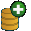
\includegraphics[width=0.7cm]{mActionAddSpatiaLiteLayer}
La primer vez que cargue datos desde una base de datos Spatialite, comienze haciendo clic en el bot\'on de la barra
de herramientas \toolbtntwo{mActionAddSpatiaLiteLayer}{A\~nadir capa de SpatiaLite} o seleccionando la opci\'on  
\dropmenuopttwo{mActionAddSpatiaLiteLayer}{A\~nadir capa de SpatiaLite...} 
del men\'u \mainmenuopt{Layer} o presionando la tecla \keystroke{L}. 
Esto mostrar\'a una ventana, la cual permitir\'a que se conecte a una base de datos Spatialite conocida por QGIS, la cual 
puede elegir del men\'u desplegable o definir una conecci\'on a una nueva base de datos. Para definir una nueva conexi\'on, haga clic en \button{Nueva} y use el navegador de archivos para apuntar hacia su base de datos SpatiaLite, 
la cual es un archivo con una extensi\'on \filename{.sqlite}.

\subsection{El di\'alogo de propiedades de vectores}\label{sec:vectorprops}
\index{vector layers!properties dialog}

El di\'alogo \dialog{Propiedades de la capa} para una capa vectorial 
provee informaci\'on acerca de la capa, configuraciones
de simbolog\'{\i}a y opciones de etiquetado. Si su capa vectorial ha sido cargada desde
un almacen de datos PostgreSQL / PostGIS, también puede alterar el SQL subyacente para la
capa - bien manualmente editando el SQL en la pesta\~na \tab{General} o invocando
el di\'alogo \dialog{Constructor de consultas} en la pesta\~na \tab{General}. 
Para accesar al di\'alogo
\dialog{Propiedades de la capa}, haga doble clic en un capa en la leyenda o clic derecho sobre
la capa y seleccione \dropmenuopt{Propiedades} del men\'u emergente.

\begin{figure}[H]
   \begin{center}
   \caption{Di\'alogo de Propiedades de Capas Vectoriales \nixcaption}\label{fig:vector_symbology}\smallskip
   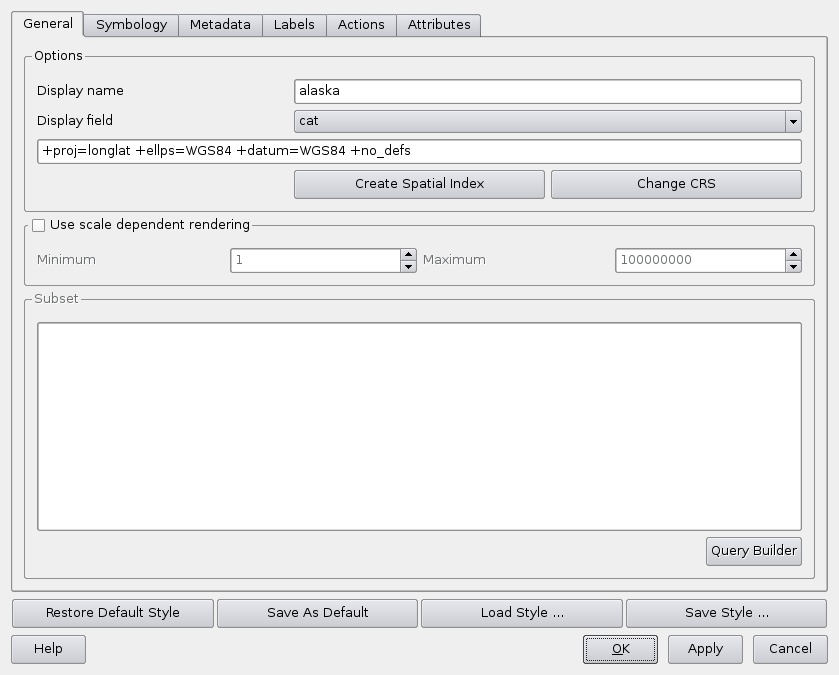
\includegraphics[clip=true, width=12cm]{vectorLayerSymbology} 
\end{center}  
\end{figure}

\subsubsection{Pesta\~na general}\label{vectorgeneraltab}
La pesta\~na \tab{General} es esencialmente muy parecida a la del di\'alogo raster. Permite
cambiar el nombre a mostrar, establecer las opciones de presentado dependientes de la escala, crear un \'{\i}ndice espacial 
de el archivo vectorial (solo para formatos OGR soportados y PostGIS) y ver o cambiar
la proyecci\'on para la capa vectorial espec\'{\i}fica.

El bot\'on \button{Constructor de consultas} le permite crear un subconjunto de caracter\'{\i}sticas 
en la capa - pero este bot\'on actualmente solo est\'a disponible cuando abre la tabla  
de atributos y selecciona el bot\'on \button{...} siguiente a b\'usqueda avanzada.

\subsubsection{Pesta\~na simbolog\'{\i}a}\label{sec:symbology}
\index{vector layers!symbology}

QGIS soporta un n\'umero de simbolog\'{\i}as de presentaci\'on para controlar como
los caracter\'{\i}sticas vectoriales son mostradas. Actualmente los siguientes presentadores
est\'an disponibles:

\begin{description} 
    \item[S\'{\i}mbolo simple] - un solo estilo es aplicado a
    cada objeto en la capa.\index{vector layers!renderers!single symbol}
    \item[S\'{\i}mbolo graduado] - los objetos dentro de la capa son
    mostrados con diferentes s\'{\i}mbolos clasificados por los valores de un
    campo particular. \index{vector layers!renderers!graduated symbol}
    \item[Color cont\'{\i}nuo] - los objetos dentro de la capa son
    mostrados con una propagaci\'on de colores clasificado por los valores
    n\'umericos de un campo espec\'{\i}fico.\index{vector layers!renderers!continuous
color}
    \item[Valor \'unico] - los objetos son clasificados por los valores \'unicos
    dentro de un campo especificado teniendo cada valor un s\'{\i}mbolo diferente.
    \index{vector layers!renderers!unique value}
\end{description}

Para cambiar la simbolog\'{\i}a de una capa, simplemente haga doble clic en su entrada
en la leyenda y el di\'alogo \dialog{Propiedades de la capa} ser\'a mostrado.\index{symbology!changing}

\begin{figure}[h]
\centering
\caption{Opciones de simbolizaci\'on \nixcaption}
   \subfigure[S\'{\i}mbolo simple] {\label{subfig:single_symbol}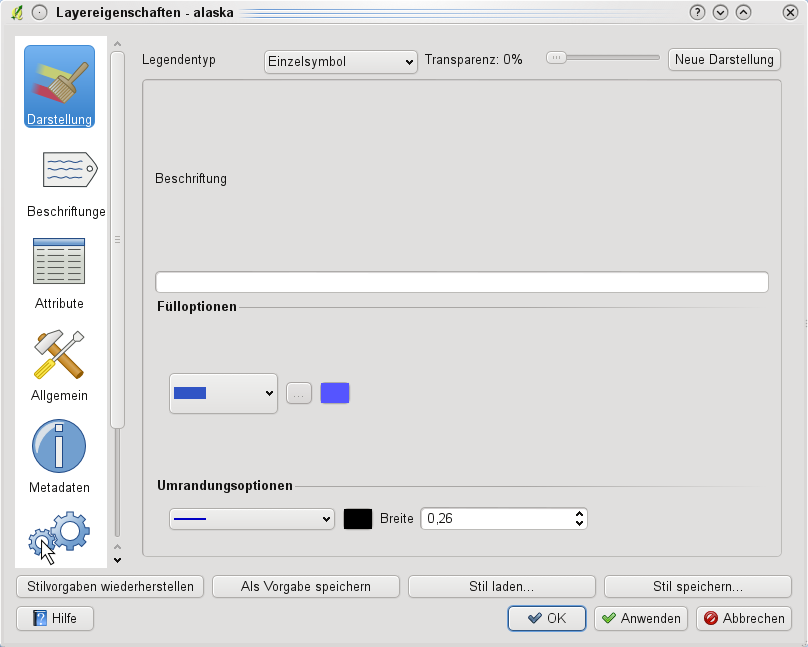
\includegraphics[clip=true, width=0.4\textwidth]{vectorClassifySingle}}\goodgap
   \subfigure[S\'{\i}mbolo graduado] {\label{subfig:graduated_symbol}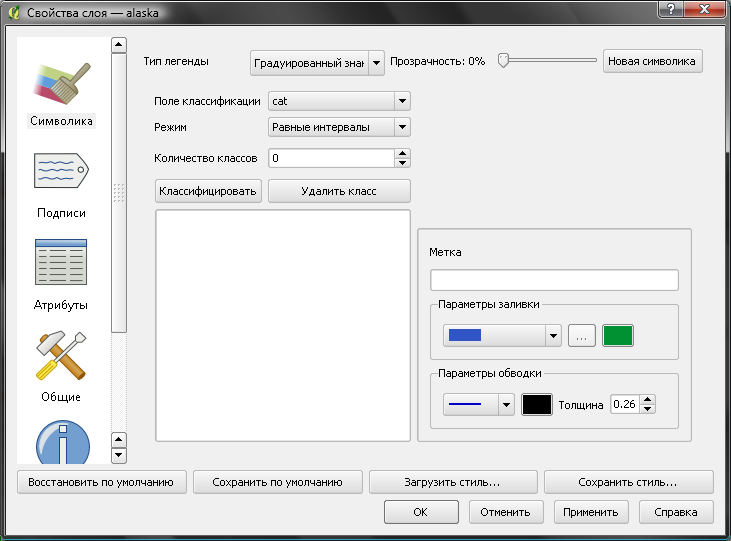
\includegraphics[clip=true, width=0.4\textwidth]{vectorClassifyGraduated}}\\
   \subfigure[Color cont\'{\i}nuo] {\label{subfig:cont_color}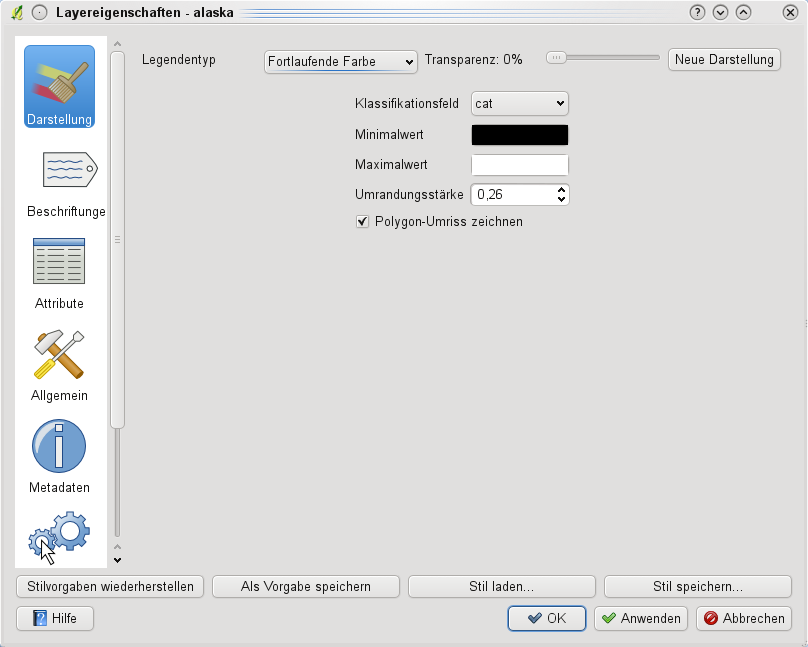
\includegraphics[clip=true, width=0.4\textwidth]{vectorClassifyContinous}}\goodgap
   \subfigure[Valor \'unico] {\label{subfig:unique_val}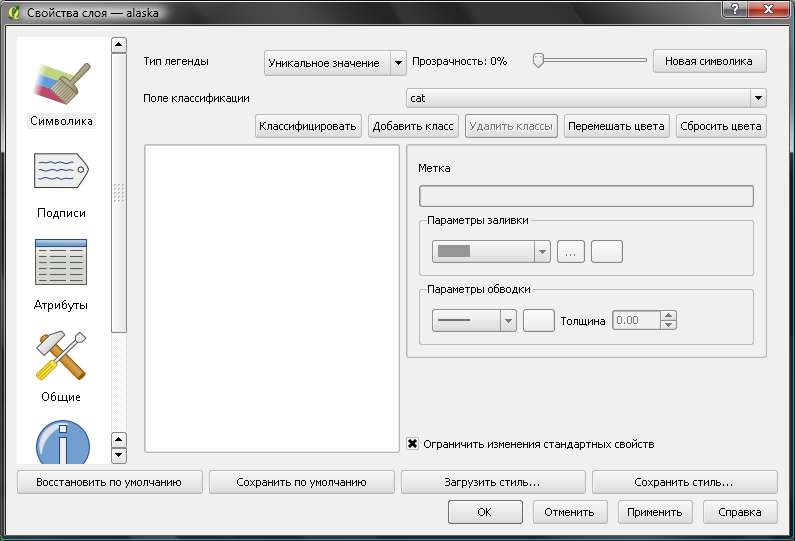
\includegraphics[clip=true, width=0.4\textwidth]{vectorClassifyUnique}}
\end{figure}

% FIXME: outdated
% Since \usertext{version v0.9} there is a function to use image files stored on 
% your computer as fill pattern for vector layers.

\minisec{Opciones de estilo} \label{sec:style_options} \index{vector layers!styles}
Dentro de este di\'alogo puede estilizar su capa vectorial. Dependiendo de la opci\'on de presentado
seleccionada tiene la posibilidad de clasificar sus caracter\'{\i}sticas del mapa.

Al menos las siguientes opciones de estilo pueden aplicarse para casi todos los presentadores:
\begin{description}
 \item[Estilo de l\'{\i}nea exterior] - estilo de lapiz para la l\'{\i}nea exterior de las caracter\'{\i}sticas. también puede establecer
 esto a 'sin lapiz'.
 \item[Color de l\'{\i}nea exterior] - color de l\'{\i}nea exterior de las caracter\'{\i}sticas.
 \item[Ancho de de l\'{\i}nea exterior] - ancho de la l\'{\i}nea exterior de las caracter\'{\i}sticas.
 \item[Color de relleno] - color de relleno de las caracter\'{\i}sticas.
 \item[Estilo de relleno] - estilo para el relleno. Aparte de las brochas definidas puede
 seleccionar \selectstring{Estilo de relleno}{? textura} y hacer clic en el bot\'on \browsebutton
 para seleccionar su propio estilo de relleno. Actualmente los formatos soportados son
 \filename{*.jpeg, *.xpm, and *.png}.
\end{description}

Una vez que ha estilizado su capa también puede almacenar su estilo de capa a
un archivo separado (con extensi\'on \filename{*.qml}).
Para hacer esto, use el bot\'on \button{Guardar estilo \ldots}. No hay necesidad de decir que
\button{Cargar estilo \ldots} carga el archivo de estilo previamente almacenado.

Si desea usar un estilo particular siempre que la capa es cargada, 
use el bot\'on \button{Guardar como predeterminado} para hacer su estilo el predeterminado. también, 
si hace cambios al estilo con los cuales no esta contento, use el bot\'on \button{Restaurar 
Estilo Predeterminado} para revertir a su estilo predeterminado.

\minisec{Transparencia de vectores} \label{sec:vect_transparency} \index{vector layers!transparency}
QGIS \CURRENT permite establecer una transparencia para cada capa vectorial. Esto puede ser hecho con
la barra de desplazamiento \slider{Transparencia}{0}{20mm} dentro de la pesta\~na \tab{symbolog\'{\i}a} (vea la fig. \ref{fig:vector_symbology}).
Esto es muy \'util para sobreponer varias capas vectoriales.

\subsubsection{Pesta\~na metadatos}

La pesta\~na \tab{Metadatos} contiene informaci\'on acerca de la capa, incluyendo peculiaridades
acerca del tipo, localizaci\'on, n\'umero de caracter\'{\i}sticas, tipo de caracter\'{\i}stica, y las capacidades de edici\'on.
La Secci\'on \guiheading{Sistema de Referencia Espacial de la Capa}, provee 
informaci\'on de proyecci\'on, y la secci\'on \guiheading{Informaci\'on de Campos de Atributos},
listados de campos y sus tipos de datos, son mostrados en esta pesta\~na. Esta es una forma r\'apida de obtener informaci\'on acerca de la capa.

\subsubsection{Pesta\~na etiquetas}

La pesta\~na \tab{Etiquetas} permite activar el etiquetado de caracter\'{\i}sticas y controlar un n\'umero de opciones
relacionadas con las fuentes, colocaci\'on, estilo, alineaci\'on y buffering.

Ilustraremos esto etiquetando el archivo shape lakes de el 
\filename{qgis\_example\_dataset}:

\begin{enumerate}
\item Cargar el archivo shape \filename{alaska.shp} y el archivo GML \filename{lakes.gml} en QGIS.
\item Ac\'erquese un poco a su \'area favorita con alg\'un lago.
\item Haga \filename{lakes} la capa activa.
\item Abra el di\'alogo \dialog{Propiedades de la capa}.
\item Clic en la pesta\~na \tab{Etiquetas}.
\item Verifique la caja de verificaci\'on \checkbox{Mostrar etiquetas} para activar el etiquetado.
\item Elija el campo con cual etiquetar. 
  Usaremos \selectstring{Campo que contiene la etiqueta}{NAMES}.
\item Escriba un valor predeterminado para lakes que no tengan nombre. La etiqueta predeterminada ser\'a
  usada cada vez que QGIS encuentre un lago sin valor en el campo \guilabel{NAMES}.
\item Si tiene etiquetas que se extienden sobre varias l\'{\i}neas, verifique \checkbox{?`Etiquetas Multil\'{\i}nea?}. 
QGIS verificar\'a una verdadera l\'{\i}nea sea regresada en su campo etiqueta e inserta retornos de l\'{\i}nea como corresponda.
Una verdadera l\'{\i}nea regresada es un caracter \textbf{simple} \textbackslash n, 
(no dos caracteres separados, como una diagonal invertida \textbackslash ~seguida del caracter n).
\item clic en el bot\'on \button{Aplicar}.
\end{enumerate} 

Ahora tenemos etiquetas. ?`C\'omo se ven? Probablemente muy grandes y pobremente colocadas en relaci\'on al s\'{\i}mbolo
marcador para los lagos.

Seleccione la entrada \tab{Fuente} y use los botones  \button{Fuente} y \button{Color}
para establecer la fuente y el color. también puede cambiar el \'angulo y la posici\'on de la etiqueta de texto.


Para cambiar la posici\'on del texto relativo a la caracter\'{\i}stica:

\begin{enumerate} 
\item Hacen clic en la entrada \tab{Fuente}.
\item Cambiar el posicionamiento seleccionando uno de los botones de selecci\'on
en el grupo \classname{Ubicaci\'on}. Para fijar las etiquetas, elija el bot\'on de selecci\'on
\radiobuttonon{Derecha}.
\item el \classname{Unidades del tama\~no de fuente} permite seleccionar entre
\radiobuttonon{Puntos} o \radiobuttonon{Unidades del mapa}.
\item Haga clic \button{Aplicar} para ver los cambios sin cerrar el di\'alogo.
\end{enumerate} 

Las cosas estan viendose mejor, pero las etiquetas todavia est\'an muy cerca a el marcador. Para
arreglar esto podemos usar las opciones en la entrada \tab{Posici\'on}. Aqu\'{\i} podemos agregar 
desplazamientos en las direcciones X y Y. Agregando un desplazamiento de 5 mover\'a las etiquetas
fuera del marcador y las har\'a más legibles. Claro si su s\'{i}mbolo marcador
o fuente es muy grande, más de un desplazamiento ser\'a requerido.

El \'ultimo ajuste que haremos es hacer un \tab{buffer} a las etiqueta. Esto significa
poner un fondo alrededor de ellas para hacer que se vean mejor. Para hacer un buffer a las
etiquetas de lagos:

\begin{enumerate}
\item Haga clic en la entrada \tab{Margen}.
\item Haga clic en la casilla de verificaci\'on  \checkbox{?` Hacer buffer de etiquetas?} para activar el buffering.
\item Elija el tama\~no del buffer usando el spin box.
\item Elija un color haciendo clic en \button{Color} y eligiendo el color favorito
  desde el selector de colores. Puede establecer alguna transparencia para el buffer
  si lo prefiere.
\item Haga clic \button{Aplicar} para ver si los cambios le agradan.
\end{enumerate} 

Si no est\'a feliz con los resultados, afine las configuraciones y pruebe nuevamente
haciendo clic en \button{Aplicar}.

Un buffer de un 1 punto parece dar un buen resultado.
Note que puede también especificar un tama\~no de buffer en unidades de mapa si eso trabaja mejor
para usted.

Las entradas restantes en la pestan\~a \tab{Etiquetas} permiten controlar la apariencia de las
etiquetas usando atributos almacenados en la capa. Las entradas con \tab{Definido o definida por datos} permiten establecer
todos los par\'ametros para las etiquetas usando campos de la capa.

Note que la pesta\~na \tab{Etiqueta} provee \classname{Previsualizaci\'on} donde 
la etiqueta seleccionada es mostrada.

\subsubsection{Pesta\~na acciones}\index{actions}\label{label_actions}

QGIS provee la habilidad de realizar una acci\'on basada en los atributos de una
caracter\'{\i}stica. Esto puede ser usado para realizar cualquier n\'umero de acciones, por ejemplo,
correr un programa con argumentos creados a partir de los atributos de una caracter\'{\i}stica o
pasando par\'ametros a una herramienta de reportes web.

Las acciones son muy \'utiles frecuentemente desea correr una aplicaci\'on externa o ver
una p\'agina web basada en uno o más valores en su capa vectorial. Un ejemplo
is realizar una b\'usqueda basada en un valor de atributo. Este concepto es usado en la  
siguiente discusi\'on.

\minisec{Definiendo Acciones}\index{actions!defining}

Las acciones de atributos son definidas desde el di\'alogo de vectores \dialog{Propiedades de la capa}. Para definir una
acci\'on, abra el di\'alogo de vectores \dialog{Propiedades de la capa} y haga clic en la
pesta\~na \tab{Acciones}. Provea un nombre descriptivo para la acci\'on. La acci\'on por si misma
debe contener el nombre de la aplicaci\'on que ser\'a ejecutada cuando la acci\'on es invocada.
Puede agregar uno o más valores de campos de atributos como argumentos
a la aplicaci\'on. Cuando la acci\'on es invocada cualquier conjunto de caracteres que empiezan
con un \% seguido del nombre de un campo ser\'an reemplazados por el valor de ese campo.
Los caracteres especiales \%\% \index{\%\%}ser\'an reemplazados por el valor
de el campo que fue seleccionado desde identificar resultados o tabla de atributos (vea
Usar Acciones abajo).  Pueden ser usadas comillas dobles para agrupar texto dentro
de un solo argumento para el programa, script o comando. Las comillas dobles ser\'an ignoradas
si est\'an precedidas por una diagonal invertida.

Si tiene nombres de campos que son subcadenas de otros nombres de campos (ej., \usertext{col1}
y \usertext{col10}) deber\'{\i}a de indicarlo
, rodeando el nombre de campo (y el \% character) con 
corchetes (ej., \usertext{[\%col10]}). Esto prevendr\'a que el nombre de campo \usertext{\%col10}
sea confundido con el nombre de campo \usertext{\%col1} con un \usertext{0}
al final. Los par\'entesis ser\'an removidos por QGIS cuando substituya el valor del campo
. Si quiere que el campo substituido sea rodeado de corchetes,
use un segundo conjunto como estos: \usertext{[[\%col10]]}.

El di\'alogo \dialog{Identificar Resultados} incluye un elemento{\em (Derivado)} que
contiene informaci\'on relevante al tipo de capa. Los valores
en este elemento pueden ser accesados en una forma similar a los otros campos
precediendo el nombre de campo derivado  con \usertext{(Derived).}. Por
ejemplo, una capa de puntos tiene un campo \usertext{X} y \usertext{Y} y el
valor de estos puede ser usado en la acci\'on con \usertext{\%(Derived).X} y
\usertext{\%(Derived).Y}. Los atributos derivados est\'an solo disponibles desde el di\'alogo
\dialog{Identificar Resultados}, y no en el di\'alogo \dialog{Tabla de atributos}.

Dos ejemplos de acciones se muestrab abajo:\index{actions!examples}

\begin{itemize}
  \item \usertext{konqueror http://www.google.com/search?q=\%nam}
  \item \usertext{konqueror http://www.google.com/search?q=\%\%}
\end{itemize}

En el primer ejemplo, el navegador konqueror es invocado y  se le pasa una URL a 
abrir. La URL realiza una b\'usqueda en Google con el valor del campo \usertext{nam}
de nuestra capa vectorial. Note que la aplicaci\'on o script llamado por la acci\'on
debe estar en la ruta o debe proveer la  ruta completa. Para estar seguros, podemos
reescribir el primer ejemplo como: \usertext{/opt/kde3/bin/konqueror
http://www.google.com/search?q=\%nam}. Esto asegurar\'a que la aplicaci\'on konqueror
ser\'a ejecutada cuando la acci\'on es invocada.

El segundo ejemplo usa la notaci\'on \%\% la cual no recae en un campo en particular
para su valor. Cuando la acci\'on es invocada, el \%\% ser\'a reemplazado por
el valor del campo seleccionado en identificar resultados o tabla de atributos.

\minisec{Usar Acciones}\index{actions!using}\label{label_usingactions}
Las acciones pueden ser invocadas bien desde el di\'alogo \dialog{Identificar resultados} o el 
 di\'alogo \dialog{Tabla de atributos}. 
(Recuerde que estos di\'alogos pueden ser abiertos haciendo clic en
\toolbtntwo{mActionOpenTable}{Identificar objetos espaciales}
o
\toolbtntwo{mActionOpenTable}{Abrir tabla de atributos}.)
Para invocar una acci\'on, 
haga clic derecho en el registro
y elija la acci\'on desde el men\'u emergente. Las acciones son listadas en el men\'u
emergente por el nombre que le asign\'o cuando defin\'{\i}a las acciones. Haga clic en la acci\'on
que desea invocar.

Si est\'a invocando una acci\'on que usa la notaci\'on \%\%, haga clic derecho en el
valor del campo que desea pasar a la aplicaci\'on o script en el di\'alogo \dialog{Identificar resultados} o en el
di\'alogo \dialog{Tabla de atributos}.

Aqui est\'a un ejemplo que jala datos de una capa vectorial y los inserta
dentro de un archivo usando bash y el comando \usertext{echo} (de esta manera solo trabajar\'a
\nix o quiza \osx). La capa en cuesti\'on tiene campos para nombres de especies
\usertext{taxon\_name}, latitud \usertext{lat} y longitud
\usertext{long}. Desear\'{\i}a poder hacer
una selecci\'on espacial de las localidades y exportar estos valores de campos a
un archivo de texto para el registro seleccionado (mostrado en amarillo en el \'area de mapa de QGIS). Aqu\'{\i} est\'a
una acci\'on para lograr esto:

\begin{verbatim}
  bash -c "echo \"%taxon_name %lat %long\" >> /tmp/species_localities.txt"
\end{verbatim} 

después de seleccionar algunas localidades y correr la acci\'on en cada una, al abrir
el archivo de salida mostrar\'a algo como esto:

\begin{verbatim}
  Acacia mearnsii -34.0800000000 150.0800000000
  Acacia mearnsii -34.9000000000 150.1200000000
  Acacia mearnsii -35.2200000000 149.9300000000
  Acacia mearnsii -32.2700000000 150.4100000000
\end{verbatim} 

Como un ejercicio creamos una acci\'on que realiza una b\'usqueda en Google sobre la capa 
\filename{lakes}. Primero necesitamos determinar la URL necesaria para realizar una b\'usqueda en una
palabra clave. Esto se realiza f\'acilmente yendo al Google y haciendo una b\'usqueda
simple, y entonces agarrando la URL desde la barra de direcciones en tu navegador. Con este
peque\~no esfuerzo vemos que el formato es: \url{http://google.com/search?q=qgis},
donde \usertext{qgis} es el t\'ermino de b\'usqueda. Armado con esta informaci\'on, podemos
proceder:

\begin{enumerate}
\item Aseg\'urese que la capa \filename{lakes} est\'a cargada.
\item Abra el di\'alogo \dialog{Propiedades de la capa} haciendo doble clic en la capa en la
  leyenda o haciendo clic derecho y elija \dropmenuopt{Propiedades} del men\'u emergente.
\item Clic en la pesta\~na \tab{Acciones}.
\item Escriba un nombre para la acci\'on, por ejemplo \usertext{Google Search}.
\item Para la acci\'on, necesitamos proveer el nombre de un programa externo a
  ejecutar. En este caso, podemos utilizar Firefox. Si el programa no esta en
  su ruta, necesita proveer la ruta completa.
\item Siguiendo el nombre de la aplicaci\'on externa, agregue la URL usada para
  hacer la b\'usqueda en Google, sin incluir el t\'ermino de b\'usqueda:
  \url{http://google.com/search?q=}
\item El texto en el campo \guilabel{Action} debe ahora verse como:\\
  \usertext{firefox \url{http://google.com/search?q=}}
\item Haga clic en la lista desplegable que contiene los nombres de los campos para la
  capa \usertext{lakes}. Est\'a localizada justo a la izquierda del
  bot\'on \button{Insertar campo}.
\item De la lista desplegable, seleccione \selectstring{}{NAMES} y haga clic en \button{Insertar campo}.
\item El texto de su acci\'on ahora se ve como:\\ \usertext{firefox
  \url{http://google.com/search?q=\%NAMES}}
\item Para finalizar la acci\'on haga clic en el bot\'on \button{Insertar acci\'on}.
\end{enumerate}
 
Esto completa la acci\'on y est\'a lista para uso. El texto final de la acci\'on
debe verse como:

\begin{center}
\usertext{firefox \url{http://google.com/search?q=\%NAMES}}
\end{center}

Ahora podemos usar la acci\'on. Cierre el di\'alogo \dialog{Propiedades de la capa} y haga un acercamiento al \'area
de inter\'es. Aseg\'urese que la capa \filename{lakes} est\'a activa e identifique un
lago. En la caja de resultados ahora ver\'a que nuestra acci\'on est\'a visible:

\begin{figure}[H]
   \begin{center}
   \caption{Seleccionar caracter\'{\i}stica y elegir acci\'on \nixcaption}\label{fig:identify_action}\smallskip
   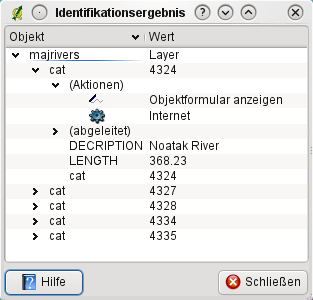
\includegraphics[clip=true, width=8cm]{action_identifyaction} 
\end{center}  
\end{figure}

Cuando hacemos clic en la acci\'on, se abre el Firefox y navega a la URL
\url{http://www.google.com/search?q=Tustumena}. también es posible agregar más 
campos de atributos a la acci\'on. Por lo tanto puede agregar un ``+'' al final del texto de la acci\'on, 
seleccionar otro campo y hacer clic en el bot\'on \button{Insertar campo}. En este ejemplo no
hay otro campo disponible que tenga sentido buscar.

Puede definir m\'ultiples acciones para una capa y cada una se mostrar\'a en el
di\'alogo \dialog{Identificar resultados}. Puede también invocar acciones desde la tabla de atributos
seleccionando una fila y haciendo clic derecho, entonces eligiendo la acci\'on desde el men\'u
emergente.

Puede pensar en todos los tipos de usos para las acciones. Por ejemplo, si tiene una capa de puntos
que contenga lugares de im\'agenes o fotos junto con un nombre de archivo, puede
crear una acci\'on para lanzar un visualizador para mostrar la imagen. también puede usar
acciones para lanzar reportes web para un campo de atributos o combinaci\'on de
campos, especific\'andolos en la misma forma que hicimos con el ejemplo de b\'usqueda en Google.

\subsubsection{Pesta\~na atributos}\index{attributes}\label{label_attributes}
Dentro de la pesta\~na \tab{Attributos} los atributos del conjunto de datos seleccionado puede ser manipulado.
Los botones \button{Nueva columna} y \button{Eliminar columna} pueden ser usados,
cuando el conjunto de datos est\'a en modo de edici\'on. Al momento solo columnas
de capas Postgis pueden ser editadas, debido a que esta funcionalidad no es soportada aun 
por la librer\'{\i}a the OGR. 

El bot\'on \button{Conmutar modo de edici\'on} activa o desactiva este modo.

\minisec{Widget de edici\'on}

Dentro de la pesta\~na \tab{Atributos} también encontrar\'a un \texttt{Widget de edici\'on} y una columna 
\texttt{valores}. Estas dos columnas pueden ser usadas para definir valores o un rango 
de valores que son permitidos para agregarse a las columnas de la tabla de atributos especifica. 
Son usadas para producir diferentes widgets de edici\'on en el di\'alogo de atributos. Estos 
widgets son:

\begin{itemize}
\item l\'{\i}nea de edici\'on: un campo de edici\'on que permite capturar texto simple (o restringir a 
n\'umeros para atributos n\'umericos).
\item valor \'unico: una lista de atributos \'unicos de las caracter\'{\i}sticas existentes
es generada y presentada en una caja de selecci\'on para su selecci\'on.
\item  valor  \'unico (editable): una combinaci\'on de `l\'{\i}nea de edici\'on' y `valor \'unico'.
El campo de edici\'on completa los valores ingresados a un valor \'unico, pero también permite
escribir valores nuevos.
\item mapa de valores: una caja de selecci\'on para seleccionar desde un conjunto de valores especificados en la
columna \texttt{value} de la pesta\~na \tab{Atributos}.  Los posibles valores son 
delimitados por un punto y coma (ej. \verb|alto;medio;bajo|). también es posible
anteponer una etiqueta a cada valor, la cual es delimitada por signo de igual (ej.
\verb|alto=1;medio=2;bajo=3|). La etiqueta es mostrada en la caja de selecci\'on en lugar
del valor.
\item clasificaci\'on: si un renderer de valor \'unico es seleccionado para la capa, los valores
usados para las clases son presentados para selecci\'on en una caja de selecci\'on.
\item rango (editable): Un campo de edici\'on que permite restringir valores n\'umericos a un
rango dado.  El rango se especifica capturando un valor m\'{\i}nimo y un valor m\'aximo
delimitado por un punto y coma(ej. \verb|0;360|) en la columna \texttt{valores} de
la pesta\~na \tab{Atributos}.
\item rango (slider): Se presenta un widget slider que permite la selecci\'on de un valor
en un rango y precisi\'on dado.  El rango es especificado por valores m\'{\i}nimo, m\'aximo
y un ancho de salto (ej. \verb|0;360;10|) en la columna \texttt{valores} de
la pesta\~na \tab{Atributos}.
\item nombre de archivo: un widget de l\'{\i}nea de edici\'on acompa\~nado de un bot\'on. Cuando se
presiona permite seleccionar un nombre de archivo usando el di\'alogo de archivo estándar.
\end{itemize}

\subsubsection{Pesta\~na diagrama}\label{sec:diagram}
\index{vector layers!diagram}

La pesta\~na \tab{Diagrama} te permite agregar un sobreposici\'on de gr\'aficos a una capa vectorial.
Para activar esta caracter\'{\i}stica, abra el Manejador de Complementos y seleccione el complemento  
de Sobreposici\'on de di\'agramas. después de esto, hay una nueva pesta\~na en el di\'alogo de vectores \dialog{Propiedades
de la capa} donde las configuraciones para los diagramas pueden ser capturadas (vea 
la figura~\ref{fig:diagramtab}).

\begin{figure}[ht]
   \begin{center}
   \caption{El di\'alogo de propiedades de vector con la pesta\~na diagramas \nixcaption}\label{fig:diagramtab}\smallskip
   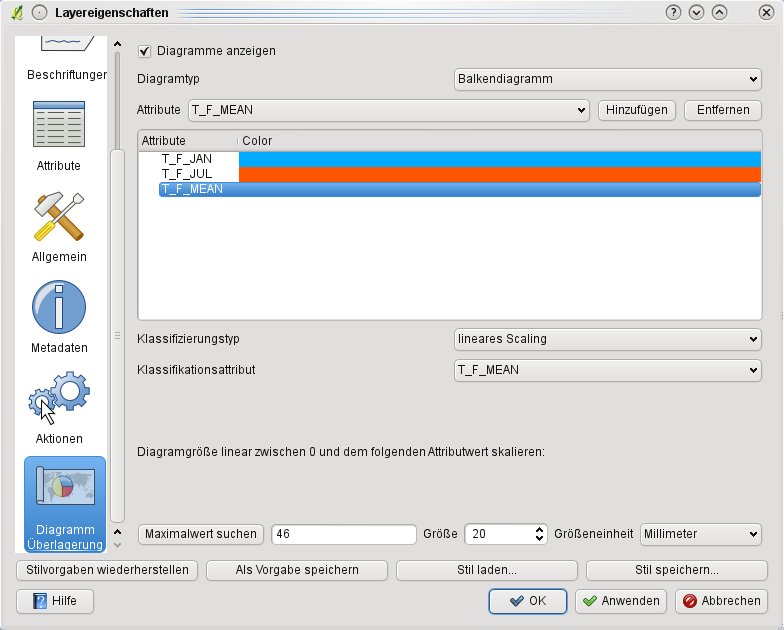
\includegraphics[clip=true, width=13cm]{diagram_tab}
\end{center}
\end{figure}

La implementaci\'on actual de di\'agramas provee soporte para barras, pastel
y para escalado lineal del tama\~no del diagrama de acuerdo a un atributo de
clasificaci\'on. Mostraremos un ejemplo la sobreposici\'on de un gr\'afico de barras
mostrando datos de temperatura desde una capa de vectores clim\'atica sobre la capa de l\'{\i}mites de Alaska.
Ambas capas vectoriales son parte del conjunto de datos de ejemplo de QGIS (vea
la Secci\'on~\ref{label_sampledata}.

\begin{enumerate}
\item Primero haga clic en el \'{\i}cono \toolbtntwo{mActionAddOgrLayer}{A\~nadir capa vectorial},
navegue hasta el directorio con el conjunto de datos de ejemplo de QGIS y cargue las dos capas de vectores
\filename{alaska.shp} y \filename{climate.shp}.
\item Haga doble clic en la capa \filename{climate} en la leyenda del mapa y abra el di\'alogo
\dialog{Propiedades de la capa}.
\item Haga clic en \tab{Sobreposici\'on de diagramas} y seleccione \button{gr\'afico de barras} como
tipo de diagrama.
\item En el diagrama queremos mostrar los valores de las tres columnas
\filename{T\_F\_JAN, T\_F\_JAN} y \filename{T\_F\_MEAN}. Primero seleccione
\filename{T\_F\_JAN} como atributos y haga clic \button{A\~nadir atributo}, entonces
\filename{T\_F\_JUL} y finalmente \filename{T\_F\_MEAN}.  
\item Para escalado lineal del tama\~no del diagrama definimos \filename{T\_F\_JUL}
como atributo de clasificaci\'on.
\item Ahora clic en \button{Encontrar valor m\'aximo}, elija un valor de tama\~no y unidad y haga clic
en \button{Aplicar} para mostrar el diagrama en la ventana principal de QGIS.
\item Ahora puede adaptar el tama\~no del gr\'afico, o cambiar los atributos de colores haciendo
doble clic en los valores de colores en el campo atributo. La
figure~\ref{fig:climatediagram} da una impresi\'on.
\item Finalmente haga clic \button{Ok}. 
\end{enumerate}

\begin{figure}[ht]
   \begin{center}
   \caption{Diagrama de datos de temperatura sobrepuesto en un mapa \nixcaption}\label{fig:climatediagram}\smallskip
   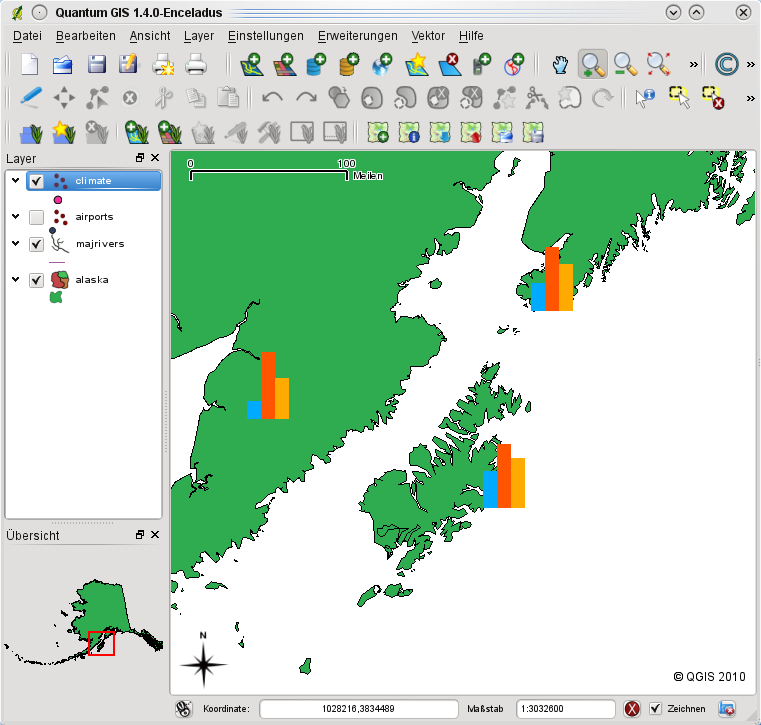
\includegraphics[clip=true, width=13cm]{climate_diagram}
\end{center}
\end{figure}

\subsection{Edici\'on}\index{editing}

QGIS suporta capacidades b\'asicas para la edici\'on de geometrias.  Antes de leer más
deber\'{\i}a notar que en esta etapa el soporte para edici\'on es preliminar.
Antes de realizar cualquier edici\'on, realize siempre una copia de respaldo del conjunto de datos
a editar. 

\textbf{Nota} - el procedimiento para editar capas de GRASS es diferente - vea la
Secci\'on \ref{grass_digitising} para detalles.

\subsubsection{Estableciendo la tolerancia de autoensamblado y radio de b\'usqueda}

Antes de poder editar v\'ertices, es muy importante establecer la tolerancia
de autoensamblado y radio de b\'usqueda a valores que nos permitan una \'optima edici\'on de
las geometr\'{\i}as de capas vectoriales. 

\minisec{Tolerancia de autoensamblado}

Tolerancia de Autoensamblado es la distancia que QGIS usa para \usertext{buscar} el v\'ertice
más cercano y/o segmento al cual trata de conectarse
cuando establece un nuevo v\'ertice o mueve un v\'ertice existente. Si no est\'a dentro
de la tolerancia de autoensamblado, QGIS dejar\'a el v\'ertice donde suelte el
bot\'on del rat\'on, en lugar de autoensamblarlo a una v\'ertice y/o segmento. 

\begin{enumerate}
\item Puede ser definida una tolerancia de autoensamblado general a lo ancho del proyecto eligiendo
\mainmenuopt{Configuraci\'on} > \dropmenuopttwo{mActionOptions}{Opciones}. 
(En Mac: vaya a  \mainmenuopt{QGIS} > Preferencias, en Linux: \mainmenuopt{Edici\'on} > \dropmenuopttwo{mActionOptions}{Opciones}.)
En la pesta\~na de \tab{Digitalizaci\'on} puede elegir entre a v\'ertice, a segmento o  a v\'ertice y
segmento como modo de autoensamblado predeterminado. también puede definir una tolerancia de
autoensamblado predeterminado y un radio de b\'usqeuda para edici\'on de v\'ertices. La tolerancia puede ser establecida bien
en unidades de mapa o en pixeles.
En nuestro proyecto de digitalizaci\'on (trabajando con el conjunto de datos de Alaska),
las unidades est\'an en pies. Sus resultados pueden variar, pero algo en el
orden de 300 pies a una escala de 1:10 000 es una configuraci\'on razonable.
\item Una tolerancia de autoensamblado basada en la capa puede ser definida eligiendo
\mainmenuopt{Configuraci\'on} (o \mainmenuopt{Archivo}) > \dropmenuopttwo{mActionOptions}{Propiedades
del proyecto\dots}. En la pesta\~na \tab{General}, en la secci\'on \classname{Digitalizaci\'on} puede hacer clic
en \button{Opciones de autoensamblado\dots} para activar y ajustar el modo de autoensamblado
y tolerancia en una capa (vea la Figura~\ref{fig:snappingoptions}).
\end{enumerate}

\begin{figure}[H]
   \begin{center}
   \caption{Editar opciones de autoensamblado para una capa \nixcaption}\label{fig:snappingoptions}\smallskip
   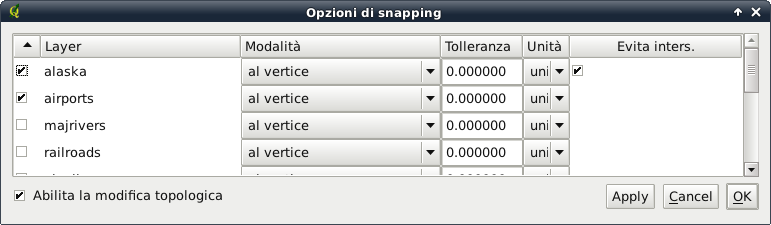
\includegraphics[clip=true, width=14cm]{editProjectSnapping} 
\end{center}  
\end{figure}

\minisec{Radio de b\'usqueda}

El radio de b\'usqueda es la distancia que QGIS usa para \usertext{buscar} el v\'ertice
más cercano que est\'a tratando de mover cuando hace clic en el
mapa. Si no est\'a dentro del radio de b\'usqueda, QGIS no encontrar\'a y seleccionar\'a
ning\'un v\'ertice para edici\'on y mostrar\'a un molesto mensaje de advertencia.
La tolerancia de autoensamblado y el radio de b\'usqueda pueden ser establecidos en unidades de mapa o pixeles, de esta manera puede
necesitar experimentar para establecerlos correctamente. Si especifica una tolerancia muy grande
QGIS puede autoensamblar al v\'ertice incorrecto, especialmente si est\'a tratando
con un gran n\'umero de v\'ertices muy proximos entre ellos. Establecer un radio de b\'usqueda muy
peque\~no no encontrar\'a nada a mover.

El radio de b\'usqueda para ediciones de vertices en unidades de capa puede ser definido en la
pesta\~na \tab{Digitalizaci\'on} bajo \mainmenuopt{Configuraci\'on} >
\dropmenuopttwo{mActionOptions}{Opciones}. El mismo lugar donde defini\'o la
tolerancia de snapping general para el proyecto.

\subsubsection{Edici\'on topol\'ogica}

Ademas de las opciones basadas en capa la pesta\~na \tab{General} en el men\'u 
\mainmenuopt{Configuraci\'on} -> \dropmenuopttwo{mActionOptions}{Propiedades del proyecto\dots} 
también provee algunas funcionalidades topol\'ogicas. 
En el grupo de opciones Digitalizaci\'on puede \checkbox{Activar edici\'on topol\'ogica} y/o activar 
\checkbox{Evitar intersecciones de nuevos pol\'{i}gonos}.

\minisec{Activar edici\'on topol\'ogica}

La opci\'on \checkbox{Activar edici\'on topol\'ogica} es para editar y mantener 
l\'{\i}mites comunes en mosaicos de pol\'{\i}gonos. QGIS "detecta" un l\'{\i}mite compartido en 
un mosaico de pol\'{\i}gonos y usted solo tiene que mover el v\'ertice una sola vez y QGIS se encargar\'a 
de actualizar el otro l\'{\i}mite.

\minisec{Evitar intersecciones de nuevos pol\'{\i}gonos}

La segunda opci\'on topol\'ogica llamada \checkbox{Evitar intersecci\'on de nuevos pol\'{\i}gonos} 
evita traslapes en mosaicos de pol\'{\i}gonos. Es para digitalizaci\'on r\'apida de pol\'{\i}gonos adyacentes. 
Si ya tiene un pol\'{\i}gono, es posible con esta opci\'on digitalizar la segunda 
de tal forma que ambas se intersecten y Qgis entonces corta el segundo pol\'{i}gono en el l\'{i}mite com\'un. 
La ventaja es que los usuarios no tienen que digitalizar todos los v\'ertices del l\'{i}mite com\'un.

\subsubsection{Edici\'on de una capa existente}
\index{vector layers!editing}
\index{editing!an existing layer}
\label{sec:edit_existing_layer}

Por defecto, QGIS carga capas como solo lectura: Esto es una medida de seguridad
para evitar editar accidentalmente una capa si hay un dezlis del mouse.
Sin embargo, puede elegir editar una capa siempre y cuando el proveedor de datos lo soporte,
y el conjunto de datos sea escribible (ej. sus archivos no son de solo escritura).

La edici\'on de capas es más versatil cuando es usada en conjuntos de datos PostgreSQL/PostGIS. 

\begin{Tip}[ht]\caption{\textsc{Integridad de datos}}
\qgistip{Siempre es una buena idea respaldar su conjunto de datos antes de iniciar 
la edici\'on. Mientras los autores de QGIS han realizado cada esfuerzo para preservar 
la integridad de sus datos, no se ofrece garant\'{\i}a en este aspecto.
}
\end{Tip}

\begin{Tip}[ht]\caption{\textsc{Manipular datos de atributos}}
\qgistip{Actualmente solo capas de PostGIS son soportadas para agregar y eliminar columnas de atributos
dentro de este di\'alogo. En versiones futuras de QGIS, otros conjuntos de datos ser\'an soportados, 
porque esta funcionalidad fue recientemente implementada en GDAL/OGR > 1.6.0
}
\end{Tip}



\begin{Tip}[ht]\caption{\textsc{Guarde regularmente}}
\qgistip{Recuerde desactivar \toolbtntwo{mActionToggleEditing}{Conmutar edici\'on} regularmente.  
Esto le permite guardar los cambios recientes,
y también confirmar que los conjuntos de datos pueden aceptar todos los cambios.
}
\end{Tip}

\begin{Tip}[ht]\caption{\textsc{Ediciones concurrentes}}
\qgistip{Esta versi\'on de QGIS no rastrea si alguien más est\'a editando un objeto espacial al mismo tiempo
que usted.  La \'ultima persona en guardar su edici\'on gana.
}
\end{Tip}

\begin{Tip}[ht]\caption{\textsc{Haga un acercamiento antes de empezar a editar}}
\qgistip{Antes de editar una capa, deber\'{\i}a hacer un acercamiento
a su \'area de inter\'es. Esto evita esperar mientras todo los marcadores de v\'ertices 
son dibujados en la capa completa.
}
\end{Tip}

\begin{Tip}[ht]\caption{\textsc{Marcadores de v\'ertices}}
\qgistip{
La versi\'on actual de QGIS soporta dos tipos de marcadores de v\'ertices 
un c\'irculo semi-transparente o una cruz. Para cambiar el estilo de marcador, elija
\dropmenuopttwo{mActionOptions}{Opciones} del men\'u
\mainmenuopt{Configuraci\'on} y haga clic en la pesta\~na \tab{Digitalizaci\'on} y seleccione
la entrada apropiada.
}
\end{Tip}

Todas las sesiones de edici\'on comienzan eligiendo la opci\'on \dropmenuopttwo{mActionToggleEditing}{Conmutar edici\'on}.
Esta puede ser encontrada en el men\'u contextual haciendo clic derecho en la entrada para esa capa en la leyenda.
\index{Allow Editing}
Alternativamente, puede usar el bot\'on \index{Conmutar edici\'on}
\toolbtntwo{mActionToggleEditing}{Conmutar edici\'on} de la barra de herramientas para empezar o parar 
el modo de edici\'on.\index{editing!icons} Una vez que la capa est\'a en modo de edic\'on, 
los marcadores aparecer\'an en los v\'ertices, y botones adicionales en la barra de herramientas 
estar\'an disponibles.

\minisec{Haciendo acercamientos, alejamientos y desplazamientos con la rueda del rat\'on}

Mientras esta digitalizando puede presionar la rueda del rat\'on para hacer un desplazamiento dentro de la ventana
principal y puede girar la rueda para acercarse o alejarse en el mapa. Para alejarse o acercarse
posicione el cursor del rat\'on dentro del \'area del mapa y gire hacia afuera (alej\'andose de usted) 
para acercarse, gire la rueda del rat\'on hacia atras (hacia usted) para alejarse. La posici\'on del cursor del rat\'on ser\'a el centro 
del acercamiento o alejamiento al \'area de inter\'es. Puede personalizar el comportamiento 
del acercamiento o alejamiento con rueda del rat\'on usando la pesta\~na \tab{Herramientas de mapa} bajo el men\'u
\mainmenuopt{Configuraci\'on} >\dropmenuopt{Opciones}.  

\minisec{Desplazamiento con las teclas de flechas}

Es posible desplazar el mapa  durante la digitalizaci\'on con las teclas de flecha. Posicione
el cursor del rat\'on dentro del \'area de mapa presione la tecla flecha derecha para hacer un
desplazamiento al este, tecla de flecha izquierda para desplazarse al oeste, tecla de flecha hacia arriba para desplazarse al norte y tecla de flecha hacia abajo 
para desplazarse al sur.

también puede usar la barra espaciadora para temporalmente causar movimientos del mouse para hacer desplazamientos 
al mapa. Las teclas ReP\'ag y AvP\'ag en su teclado causar\'an que la vista se acerque 
o aleje sin interrumpir su sesi\'on de digitalizaci\'on.

Puede realizar las siguiente funciones de edici\'ons:

\begin{itemize}
\item Agregar Objetos Espaciales: \toolbtntwo{mActionCapturePoint}{Capturar Punto},
  \toolbtntwo{mActionCaptureLine}{Capturar L\'{\i}nea} y
  \toolbtntwo{mActionCapturePolygon}{Capturar Pol\'{\i}gono}
\item \toolbtntwo{mActionAddRing}{A\~nadir Anillo}
\item \toolbtntwo{mActionAddIsland}{A\~nadir Isla}
\item \toolbtntwo{mActionSplitFeatures}{Dividir Objeto Espacial}
\item \toolbtntwo{mActionMoveFeature}{Mover Objeto Espacial}
\item \toolbtntwo{mActionMoveVertex}{Mover V\'ertice}
\item \toolbtntwo{mActionAddVertex}{Agregar V\'ertice}
\item \toolbtntwo{mActionDeleteVertex}{Borrar V\'ertice}
\item \toolbtntwo{mActionDeleteSelected}{Borrar Seleccionado}
\item \toolbtntwo{mActionEditCut}{Cortar Objeto Espacial}
\item \toolbtntwo{mActionEditCopy}{Copiar Objeto Espacial}
\item \toolbtntwo{mActionEditPaste}{Pegar Objeto Espacial}
\end{itemize}

\minisec{Agregar Objetos Espaciales}
\index{vector layers!adding!feature}

Antes de iniciar agregar objetos espaciales, use las herramientas \toolbtntwo{mActionPan}{Desplazar mapa}
y \toolbtntwo{mActionZoomIn}{Acercar zum}/\toolbtntwo{mActionZoomOut}{Alejar zum} 
para navegar al \'area de inter\'es.

Entonces tiene que usar los \'{\i}conos \toolbtntwo{mActionCapturePoint}{Capturar punto},
\toolbtntwo{mActionCaptureLine}{Capturar l\'{\i}nea} o
\toolbtntwo{mActionCapturePolygon}{Capturar pol\'{\i}gono} en la barra de herramientas para poner el cursor de QGIS
en modo de digitalizaci\'on.

Para cada objeto espacial, primero digitaliza la geometr\'{\i}a, después captura sus atributos.

Para digitalizar la geometr\'{\i}a, haga clic izquierdo en el \'area del mapa para crear el primer
punto de su nuevo objeto espacial.

Para l\'{\i}neas y pol\'{\i}gonos, siga haciendo clic izquierdo para cada punto adicional
que desee capturar. Cuando haya finalizado de agregar puntos,
haga clic derecho en cualquier parte del \'area de mapa para confirmar que ha terminado de meter
la geometr\'{i}a de ese objeto espacial.

La ventana de atributos aparecer\'a, permitiendole meter la informaci\'on del nuevo objeto espacial.
La Figura \ref{fig:vector_digitising} muestra como establecer atributos para un nuevo rio ficticio
en Alaska.

\begin{figure}[ht]
   \begin{center}
   \caption{Di\'alogo de Introducir Valores de Atributos después de digitalizar un nuevo objeto espacial vectorial
   \nixcaption}\label{fig:vector_digitising}\smallskip
   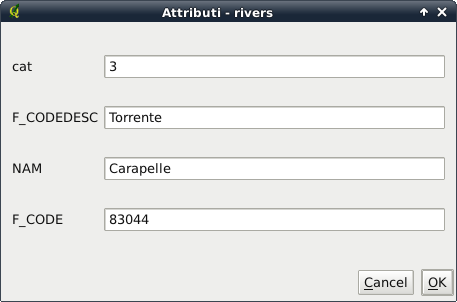
\includegraphics[clip=true, width=8cm]{editDigitizing}
\end{center}  
\end{figure}

\begin{Tip}[ht]\caption{\textsc{Tipos de Valores de Atributos}}
\qgistip{
Al menos para edici\'on de archivos shape los tipos de atributos son validados durante la
captura. Por esto, no es posible capturar un n\'umero dentro de una columna de texto en el di\'alogo
\dialog{Introducir Valores de Atributos} o viceversa. Si necesita hacerlo as\'{\i},
deber\'{\i}a editar los atributos en un segundo paso dentro del di\'alogo \dialog{Tabla
de atributos}.
}
\end{Tip}

\minisec{Mover Objeto Espacial}
\index{vector layers!move!feature}

Puede mover objetos espaciales usando el \'{\i}cono \toolbtntwo{mActionMoveFeature}{Mover Objeto Espacial} 
de la barra de herramientas.

\minisec{Dividir Objeto Espacial}
\index{vector layers!split!feature}

Puede dividir objetos espaciales usando el \'{\i}cono \toolbtntwo{mActionSplitFeatures}{Dividir Objeto Espacial}
de la barra de herramientas.

\minisec{Editar V\'ertices de un Objeto Espacial}
\index{vector layers!editing!vertex}

Para ambos tipos de capas PostgreSQL/PostGIS y  archivo shape, los v\'ertices de los objetos espaciales pueden ser editados. 

Los v\'ertices pueden ser directamente editados, esto es, no tiene
que elegir cual nuevo objeto espacial editar antes de que pueda cambiar
su geometr\'{\i}a.
En algunos casos, m\'ultiples objetos espaciales pueden compartir el mismo v\'ertice
y de esta manera las siguientes reglas aplican cuando el rat\'on es presionado
cerca de objetos espaciales del mapa:

\begin{itemize}
\item \textbf{L\'{\i}neas}    - La l{\'i}nea más cercana a la posici\'on del rat\'on
                          es usada como objeto espacial objetivo.
                          Entonces (para mover y eliminar un v\'ertice)
                          el v\'ertice más cercano
                          en esa l\'{\i}nea es el objetivo de edici\'on.

\item \textbf{Pol\'{\i}gonos} - Si el rat\'on est\'a dentro del pol\'{\i}gono, entonces ese
                          es el objeto espacial objetivo; de lo contrario el pol\'{\i}gono más cercano
                          es usado.
                          Entonces (para mover y eliminar un v\'ertice)
                          el v\'ertice más cercano
                          en ese pol\'{\i}gono es el objetivo de edici\'on.                          
\end{itemize}

Necesitar\'a establecer la propiedad
\mainmenuopt{Configuraci\'on}>\dropmenuopttwo{mActionOptions}{Opciones}>\tab{Digitalizaci\'on}>\selectnumber{Radio de b\'usqueda}{10}
a un n\'umero mayor que cero.  De lo contrario QGIS no podr\'a decir que objeto espacial est\'a siendo editado.


\minisec{Agregar V\'ertices a un Objeto Espacial}
\index{vector layers!adding!vertex}

Puede agregar nuevos v\'ertices a un objeto espacial usando el \'{\i}cono
\toolbtntwo{mActionAddVertex}{A\~nadir V\'ertice} 
de la barra de herramientas.

Note que, no tiene sentido agregar más v\'ertices a un objeto espacial puntual!

En esta versi\'on de QGIS, los v\'ertices solo pueden ser agregados a un segmento \textit{existente} 
de un objeto espacial de l\'{\i}nea.  Si quiere extender una l\'{\i}nea más all\'a de su final,
necesitar\'a primero mover el v\'ertice final, entonces agregar un nuevo v\'ertice donde
el terminal solia estar.

\minisec{Moviendo V\'ertices de un Objeto Espacial}
\index{vector layers!moving!vertex}

Puede mover v\'ertices usando el \'{\i}cono \toolbtntwo{mActionMoveVertex}{Mover V\'ertice}
de la barra de herramientas.

\minisec{Eliminar V\'ertices de un Objeto Espacial}
\index{vector layers!deleting!vertex}

Puede eliminar v\'ertices usando el \'{\i}cono \toolbtntwo{mActionDeleteVertex}{Borrar V\'ertice}
de la barra de herramientas.

Note que, no tiene sentido eliminar el v\'ertice de un objeto espacial puntual!
En lugar de eso elimine el objeto espacial completo.

Similarment, una l\'{\i}nea de un solo v\'ertice o un pol\'{\i}gono de dos v\'ertices también es
bastante inutil y llevar\'a a resultados impredecibles en alg\'un otro lugar en
QGIS, as\'{\i} que no haga eso.

\textbf{advertencia:} Un v\'ertice es identificado para eliminaci\'on tan pronto 
como hace clic con el rat\'on cerca de un objeto espacial elegible.
Para deshacerlo, necesitara desactivar
la edici\'on y después descartar sus cambios.
(Claro esto significar\'a que otros cambios sin guardar ser\'an perdidos, también.)

\minisec{A\~nadir Anillo}
\index{vector layers!add!ring}

Puede crear pol\'{\i}gonos anillo usando el \'{\i}cono \toolbtntwo{mActionAddRing}{A\~nadir Anillo}
de la barra de herramientas. Esto significa que dentro de un \'area existente es posible digitalizar
otros pol\'{\i}gonos, esto ocurrir\'a como un 'todo', de esta manera solo 
el \'area entre los l\'{\i}mites del pol\'{\i}gono más externo y el más interno permanecen 
como un pol\'{\i}gono anillo. 

\minisec{A\~nadir Isla}
\index{vector layers!add!island}

Puede \toolbtntwo{mActionAddIsland}{A\~nadir isla} a multipol\'{\i}gonos seleccionados. 
El nuevo pol\'{\i}gono isla tiene que ser digitalizado fuera del multipol\'{\i}gono seleccionado. 

\minisec{Cortar, Copiar y Pegar Objetos Espaciales}
\index{vector layers!cut!feature}
\index{vector layers!copy!feature}
\index{vector layers!paste!feature}
\index{editing!cutting features}
\index{editing!copying features}
\index{editing!pasting features}

Las objetos espaciales seleccionados pueden ser cortados, copiados y pegados entre capas en el mismo proyecto
de QGIS, siempre y cuado de antemano las capas de destino han sido establecidos a  
\toolbtntwo{mActionToggleEditing}{Conmutar edici\'on}.

Los objetos espaciales pueden también ser pegadas a aplicaciones externas como texto:  Esto es,
los objetos espaciales son presentadas en formato CSV con los datos de geometr\'{\i}a 
en el formato Well-Known Text (WKT) de la OGC.


Sin embargo en esta versi\'on de QGIS, el texto de objetos espaciales de fuera de QGIS no pueden 
ser pegadas a una capa dentro de QGIS. ?`Cu\'ando ser\'{\i}a \'util la funci\'on de copiar y pegar? 
Bien, resulta que puede editar más de una capa 
al tiempo que copia y pega caracter\'{\i}sticas entre capas. ?`Por qu\'e querriamos hacer
eso?  dicho que tenemos que hacer una trabajo sobre una nueva capa pero solo necesita uno o
dos lagos, no los 5,000 en nuestra capa \filename{big\_lakes}. Podemos crear una nueva capa
y usar copiar/pegar para soltar los lagos necesarios en ella. 

Como un ejemplo estamos copiando algunos lagos a una nueva capa:

\begin{enumerate}
\item Cargue la capa de la que desea copiar (capa fuente)
\item Cargue o cree la capa a la que desea copiar (capa destino) 
\item Inicie la edici\'on para la capa destino
\item Haga la capa fuente activa haciendo clic en ella en la leyenda 
\item Use la herramienta \toolbtntwo{mActionSelect}{Seleccionar} para seleccionar el objeto espacial(es) en la capa fuente
\item Haga clic en la herramienta \toolbtntwo{mActionEditCopy}{Copiar  Objetos Espaciales}
\item Haga la capa destino activa haciendo clic en ella en la leyenda 
\item Haga clic en la herramienta \toolbtntwo{mActionEditPaste}{Pegar Objetos Espaciales}
\item Pare la edici\'on y guarde los cambios
\end{enumerate}

?`Qu\'e pasa si las capas fuentes y destino tienen
diferentes esquemas (no son iguales los nombres de campos y tipos)? QGIS llena
lo que coincide e ignora el resto. Si no le interesa los atributos
siendo copiados a la capa destino, no importa como dise\~ne los
campos y los tipos de datos. Si desea asegurarse que todo - objetos espaciales y sus
atributos - son copiados, aseg\'urese que los esquemas coincidan.

\begin{Tip}[ht]\caption{\textsc{Congruencia de Objetos Espaciales Pegados}}
\qgistip{Si sus capas de fuente y destino usan la 
misma proyecci\'on, entonces los objetos espaciales pegados tendr\'an
una geometr\'{\i}a id\'entica a la capa fuente.
Sin embargo si la capa destino tiene una proyecci\'on diferente
entonces QGIS no puede garantizar que la geometr\'{\i}a es identica.
Esto es simplemente porque hay peque\~nos errores de redondeo
involucrados durante la conversi\'on entre proyecciones.
}
\end{Tip}

\minisec{Eliminado Objetos Espaciales Seleccionados}
\index{vector layers!deleting!feature}

Si deseamos eliminar un pol\'{\i}gono completo, podemos hacerlo primero seleccionando 
el pol\'{\i}gono usando la herramienta regurl \toolbtntwo{mActionSelect}{Seleccionar Objetos Espaciales}. Puede seleccionar 
m\'ultiples objetos espaciales para su eliminaci\'on. Una vez que ha establecido la selecci\'on, use la 
herramienta \toolbtntwo{mActionDeleteSelected}{Borrar lo Seleccionado} para eliminar los objetos espaciales. No hay funci\'on deshacer, 
pero recuerde que su capa no ha cambiado realmente hasta que pare la edici\'on y elija 
guardar los cambios. De esta manera si comete alg\'un error, siempre puede cancelar el guardar.

La herramienta \toolbtntwo{mActionEditCut}{Cortar Objetos Espaciales} en la barra de herramientas de digitalizaci\'on también puede
ser usada para eliminar objetos espaciales. Esto efectivamente elimina los objetos espaciales pero
también la coloca en un lugar especial llamado ``portapapeles espacial". De esta manera cortamos el objetos espacial a eliminar. 
Podemos entonces usar la \toolbtntwo{mActionEditPaste}{Herramienta pegar} para regresarla, d\'andonos la funcionalidad de deshacer de un nivel. 
Cortar, copiar, y pegar trabajan sobre los objetos espaciales seleccionados actualmente, 
significando que podemos operar en más de uno al mismo tiempo.

\begin{Tip}[ht]\caption{\textsc{Soporte para la Eliminaci\'on de Objetos Espaciales}}
\qgistip{Cuando se edita ESRI archivos shape, el borrado
de objetos espaciales solo trabaja si QGIS est\'a compilado con una versi\'on de GDAL version 1.3.2 o superior. 
Las versiones de QGIS para OS X y Windows disponibles en el sitio de descarga estan compilados 
usando GDAL 1.3.2 o superior.
}
\end{Tip}

\minisec{Modo Autoensamblado}
\index{editing!snap}
QGIS permite que los v\'ertices digitalizados sean autoensamblados a otros v\'ertices de la misma capa. Para 
establecer la tolerancia de autoensamblado, vaya a
\mainmenuopt{Configuraci\'on}>\dropmenuopttwo{mActionOptions}{Opciones}->\tab{Digitalizaci\'on}.
(En Mac: vaya a  \mainmenuopt{QGIS} > Preferencias, En Linux: \mainmenuopt{Editar} > \dropmenuopttwo{mActionOptions}{Opciones}.)
Note que la tolerancia de autoensamblado est\'a en unidades de mapa o pixeles.

\minisec{Guardar Capas Editadas}
\index{editing!saving changes}

Cuando una capa est\'a en modo de edici\'on, cualquier cambio permanece pendiente en la memoria de QGIS.
Por lo tanto no se guardan o se les aplica un commit inmediatamente al conjunto de datos o disco.
Cuando desactiva la edici\'on (o sale de QGIS para el caso), 
se le pregunta si desea guardar sus cambios o
descartarlos.

Si los cambios no pueden ser guardados (ej. disco lleno, o los atributos tienen
valores fuera de rango), el estado de memoria de QGIS es preservado.  Esto
permite que ajuste su edici\'on y lo intente de nuevo.

\subsubsection{Crear una nueva capa}\label{sec:create shape}\index{editing!creating a new layer}

Para crear una nueva capa para edici\'on, elija \toolbtntwo{mActionNewVectorLayer}{Nueva Capa Vectorial} del
 men\'u \mainmenuopt{Capa}. 
Se mostrar\'a un dia\'alogo \dialog{Nueva Capa Vectorial} como el de la
Figura \ref{fig:newvectorlayer}. Elija el tipo de capa (punto,
l\'{\i}nea o pol\'{\i}gono).

\begin{figure}[ht]
   \begin{center}
   \caption{Di\'alogo nueva capa vectorial \nixcaption}\label{fig:newvectorlayer}\smallskip
   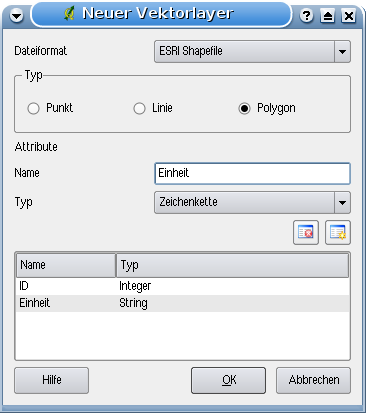
\includegraphics[clip=true, width=10cm]{editNewVector}
\end{center} 
\end{figure}

Note que QGIS no soporta aun la creaci\'on de
objetos espaciales 2.5D (ej. objetos espaciales con coordenadas X,Y,Z) o objetos espaciales de medidas.
A la fecha solo pueden ser creados archivos shape. En una futura versi\'on de QGIS, la creaci\'on de cualquier tipo
de capa OGR o PostgreSQL ser\'a soportado. 

La creaci\'on de capas GRASS es soportada dentro del complemento de GRASS. Vea la secci\'on 
\ref{sec:creating_new_grass_vectors} para más informaci\'on de creaci\'on de capas GRASS.

Para completar la creaci\'on de una nueva capa, agregue los atributos deseados haciendo
clic en el bot\'on  \button{A\~nadir atributo} y especificando un campo y el tipo para al atributo.
Solo los tipos de atributos \selectstring{Tipo}{real}, \selectstring{Tipo}{entero}, y \selectstring{Tipo}{cadena} son soportados. Una vez que esta contento con sus atributos,
haga clic en \button{OK} y provea un nombre para el archivo shape.
QGIS autom\'aticamente agregar\'a una extensi\'on \filename{.shp} al nombre que especific\'o. Una vez
que la capa ha sido creada, ser\'a agregada al mapa y puede ser editada en la misma forma
que se describe en la Secci\'on anterior \ref{sec:edit_existing_layer}. 

\subsubsection{Trabajar con la tabla de atributos}\label{sec:attribute table}\index{editing!working with the attribute table}

Para abrir la tabla de atributos para una capa vectorial, active la capa haciendo clic en ella en el \'area de leyenda del mapa. 
Entonces use el men\'u  capa\mainmenuopt{Capa} del men\'u principal y elija \dropmenuopttwo{mActionOpenTable}{Abrir tabla de atributos} 
desde el men\'u. también es posible hacer clic derecho en la capa y elegir \dropmenuopttwo{mActionOpenTable}{Abrir Tabla de Atributos} 
desde el men\'u desplegable. Esto abrir\'a una nueva ventana que mostrar\'a los atributos para cada objeto espacial en la capa 
(figure \ref{fig:attributetable}).

\begin{figure}[ht]
   \begin{center}
   \caption{Tabla de atributos para la tabla de Alaska \nixcaption}\label{fig:attributetable}\smallskip
   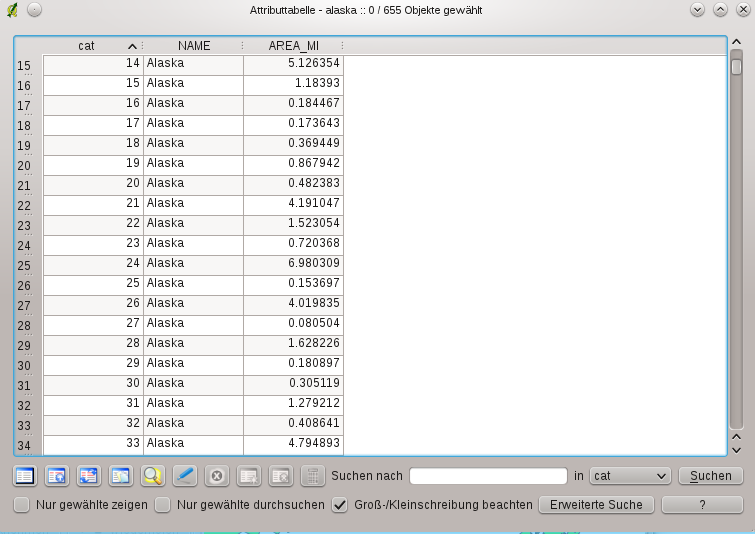
\includegraphics[clip=true, width=12cm]{vectorAttributeTable}
\end{center} 
\end{figure}

Cada columna puede ser ordenada haciendo clic en su encabezado. Una peque\~na flecha indica el orden 
(apuntando hacia abajo significa valores descendentes de la primara columna hacia abajo, apuntando hacia arriba significa valores ascendentes desde la primera columna hacia abajo). 
Para una selecci\'on simple de atributos en una columna el bot\'on \button{Buscar en} 
puede ser usado. Seleccione el campo (columna) en la cual la b\'usqueda ser\'a realizada 
de la caja de selecci\'on y presione el bot\'on \button{Buscar}. Para b\'usquedas más complejas use
el bot\'on B\'usquedas Avanzadas \button{...}, el cual lanzar\'a el Constructor de Consultas de B\'usqueda descrito en 
la Secci\'on \ref{sec:select_by_query}. 

Para solo mostrar los registros, use la caja de selecci\'on \checkbox{Mostrar solo los registros seleccionados}.
Usando los botones en la parte inferior izquierda  de la ventana, campos seleccionados pueden ser removidos, 
movidos a la parte superior de la tabla, o la selecci\'on puede ser invertida. Los objetos espaciales seleccionados también pueden ser
copiadas al portapapeles, que también puede ser hecho con \keystroke{Ctrl-C}. Puede hacer zoom 
a los objetos espaciales seleccionados en el mapa. Conmutar la edici\'on permite editar valores de atributos. 

\subsection{Constructor de consultas}\label{sec:query_builder}
\index{Query Builder}

El Constructor de Consultas permite definir un subconjunto de una tabla y mostrarlo como una capa en QGIS. Actualmente solo puede ser usado con capas PostGIS. 
Por ejemplo, si se tiene una capa \filename{towns} con un campo \usertext{population} puede seleccionar solo ciudades grandes escribiendo \usertext{population > 100000} en la caja SQL del constructor de consultas. Figura
\ref{fig:query_builder} muestra un ejemplo del constructor de consultas llenado con datos de una capa PostGIS con atributos almacenada en PostgreSQL. 

\begin{figure}[ht]
  \begin{center}
    \caption{Query Builder \nixcaption}\label{fig:query_builder}\smallskip
    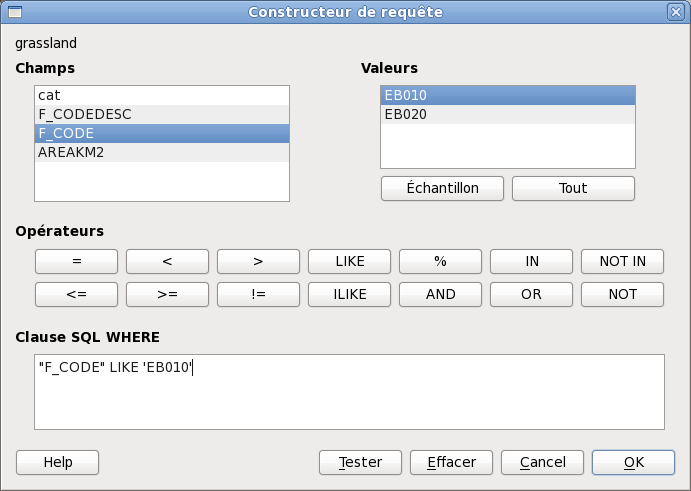
\includegraphics[clip=true, width=11.5cm]{queryBuilder}
  \end{center}  
\end{figure}

El constructor de consultas \index{Query Builder} lista los campos de la capa de la base de datos en una lista en la izquierda. Puede obtener un ejemplo de los datos contenidos en el campo resaltado haciendo clic en el bot\'on \button{Sample} \index{Query
Builder!generating sample list}. Esto recupera los primeros 25 valores distintos para el campo desde la base de datos. Para obtener una lista de todos los posibles valores para un campo, haga clic en el bot\'onf \button{Todos} \index{Query Builder!getting all
values}. Para agregar un campo seleccionado o valor a la consulta, haga doble clic en el\index{Query Builder!adding fields}. Puede usar varios botones para construir la consulta o puede escribirla dentro de la caja SQL.

Para probar una consulta, haga clic en el bot\'on \button{Probar} \index{Query Builder!testing
queries}. Esto regresar\'a un conteo del n\'umero de registros que pueden ser incluidos en la capa. Cuando est\'e satisfecho con la consulta, haga clic en el bot\'on \button{OK}. El SQL para la clausula where ser\'a mostrada en la columna SQL de la lista de capas.

\begin{Tip}\caption{\textsc{Cambiar la Definici\'on de la Capa}}\index{Query
Builder!changing layer definitions}
\qgistip{Puede cambiar la definici\'on de la capa después de que es cargada alterando
la consulta SQL usada para definir la capa. Para hacer esto, abra el 
di\'alogo  de vectores \dialog{Propiedades de la capa} haciendo doble clic en la capa en la leyenda y clic en el bot\'on
\button{Constructor de Consultas} en la pesta\~na \tab{General}. Vea la secci\'on
\ref{sec:vectorprops} para más informaci\'on.}
\end{Tip}

\subsection{Selecci\'on por consulta}\label{sec:select_by_query}
\index{PostgreSQL!query builder}
\index{PostGIS!query builder}
\index{query builder!PostgreSQL}
\index{query builder!PostGIS}

Con QGIS también es posible seleccionar objetos espaciales usando una interface similar al constructor de consultas utilizado en \ref{sec:query_builder}. En la secci\'on superior el prop\'osito del constructor de consultas es solo mostrar los objetos espaciales cumpliendo el filtro como una 'capa virtual'/subconjunto. El prop\'osito de la funci\'on seleccionar por consulta es resaltar todas los objetos espaciales que cumplan con un criterio particular. Seleccionar por consulta puede ser usado con todos los proveedores de datos.

Para hacer una 'selecci\'on por consulta' en una capa cargada, haga clic en el bot\'on \toolbtntwo{mActionOpenTable}{Abrir tabla de atributos} para abrir la tabla de atributos de la capa. Entonces clic en el bot\'on \button{Avanzado...} en la parte inferior. Esto inicia el Constructor de Consultas que permite definir un subconjunto de una tabla y mostrarlo como se describe en la Secci\'on \ref{sec:query_builder}.


\index{vector layers|)}
